\chapter{2023年}

\section{1月}

\subsection*{2023年01月06日 12:33}
\addcontentsline{toc}{subsection}{2023年01月06日 12:33}

\url{https://youtu.be/9dpuVMdUutM}

\paragraph{リンク}
\url{https://youtu.be/9dpuVMdUutM}

\subsection*{2023年01月13日 21:29}
\addcontentsline{toc}{subsection}{2023年01月13日 21:29}

\url{https://youtu.be/LAaakVWnrXg}

新年を大好きなワルツでスタートする事ができました。

ウィーンフィルが演奏するウィンナワルツの話じゃありません。

ラヴェルのワルツです。木琴、鉄琴、グロッケンなどなど、色んな打楽器を使っての編曲ですが、面白いです。いいですね〜。

\paragraph{リンク}
\url{https://youtu.be/LAaakVWnrXg}

\subsection*{2023年01月20日 19:14}
\addcontentsline{toc}{subsection}{2023年01月20日 19:14}

話題のシステムと少し対話してみた。

どこまで信じられるのかわかりませんが、極めてまともな文章(文ではない)が出力されるのは確かです。（すごい！）

Googleでググっていると思えば、最低でもその程度には使えるんだろうという気はしていますし、むしろ、Googleなどの検索ボックスの形のインターフェースは、これと置き代わっていくかもしれないという気さえします。

それにしても、この手のシステムに接して思い出すのは、Elizaという（往年の）対話システム（\url{https://ja.m.wikipedia.org/wiki/ELIZA}）です。Doctorという別名でも呼ばれていました。（Elizaという命名の元は、ミュージカル「マイ・フェア・レイディ」の主人公の名前です。映画ではオードリ・ヘプバーンが主演でした。「スペインの雨は主に荒野に降る‥」）学生だった頃、bitという雑誌（共立出版）にLispで記述されたEliza の処理系の話が載っていて、とても興味を持った記憶があります。

Elizaに比べると、ChatGPTは寡黙で偉そうですね。質問を入力するための空欄があるだけですから。たしかElizaだったら「どうしたの」とか「そのことについてもう少し話して下さい」みたいな、Doctorっぽい、心理カウンセラっぽい、それらしい事を言ってきたように記憶しています。（ChatGPTのAPIが公開されれば、すぐにもDoctorの進化版の様なものも出てくるかもしれません。）

かのアラン・チューリングが人工知能について「コンピュータの向こう側からの応答が、人なのかコンピュータなのか区別がつかなかったなら、そのコンピュータシステムには知能があると言える」という様な事を言ったとか。（これも当時のbit誌から得た断片的な知識なので、うろ覚えですが）Doctorはその辺りを目指していたのでしょうね。（近年では「人工知能」という４字熟語には古典的な響きを感じます。トレンドは「AI」でしょうか。）

ChatGPTが応答してくれる内容について、盲目的に信頼するつもりはありません。しばらくは斜め目線で接していきたいと思いますが、少なくとも自然言語処理の進化については、顕著なものがあるようです。

ここを見るとあっという間にElizaっぽくなってきている。

\url{https://twitter.com/nikkei_linux/status/1625692702749892608?s=61&t=jlXc1DUVYsfXAuxxJQ9a_g}

\paragraph{リンク}
\url{https://openai.com/blog/chatgpt/}

\subsection*{2023年01月29日 20:25}
\addcontentsline{toc}{subsection}{2023年01月29日 20:25}

「プログラミング技術」という教科書（実教）を使っている科目（工業高校2年生）の授業ですが、この教科書は最初から最後までC言語の詳しい学習書になっています。これを一年間勉強をしてきたので、一段落として「少しだけ長めのプログラムで、ゲームなんかどう？」という事で用意した資料です。

以下のGitHubのreadmeフォルダにドキュメントとしてCUIGamesWithC.pdfとそれを書いたTeXのソースを置いています。また、srcフォルダには、実際に動作させてみたC言語のソースプログラムなどを置いています。

\#C言語 \#GitHub \#tictactoe \#TeX \#slidetile \#flipcard \#Game

\paragraph{リンク}
\url{https://github.com/smat1957/CLanguageCUIGames}

\subsection*{2023年01月29日 20:48}
\addcontentsline{toc}{subsection}{2023年01月29日 20:48}

「ハードウェア技術」という教科書（実教）を使っている同名の科目の授業（工業高校3年生）で、アセンブラによる論理演算を扱っている所です。

「皆んなが2年生の時に勉強してきたC言語でも、ここで扱っているアセンブラと同様のビット操作、論理演算ができるんだよ」ということを示すために用意したA4裏表一枚の資料です。10bitのAD変換器からデータを読み込む例を、この資料の最終目標に置いています。

それにしても、昔のCPUのレジスタなら、こんな長い2進bit列を見なくて済むのに、と思いながら書いていました。何とか意味のある一行に納めて、見やすい2進bit列になる様工夫しているつもりです。

資料は以下のGitHubにて。readmeフォルダ以下のcLogic.pdfで公開します。このドキュメントを作成したTeXのソースも、同じファイル名（拡張子はTeX）で、同じフォルダに置いています。なお、src フォルダには実際に動作させてみたC言語のソースプログラムclogic.cなども置いています。

\#C言語 \#アセンブラ \#CPU \#AD変換 \#GitHub \#TeX \#論理演算

\paragraph{リンク}
\url{https://github.com/smat1957/CLanguageBitOperation}

\section{2月}

\subsection*{2023年02月16日 02:25}
\addcontentsline{toc}{subsection}{2023年02月16日 02:25}

あっという間にElizaっぽくなってきた。

\paragraph{リンク}
\url{https://twitter.com/nikkei_linux/status/1625692702749892608?s=12&t=jlXc1DUVYsfXAuxxJQ9a_g}

\subsection*{2023年02月28日 22:33}
\addcontentsline{toc}{subsection}{2023年02月28日 22:33}

今日の富山市です。職場の近くで撮影。

昨日もそうでしたが、立山連峰が美しい。

\paragraph{写真}
\begin{center}
\begin{minipage}{0.70\linewidth}
\centering
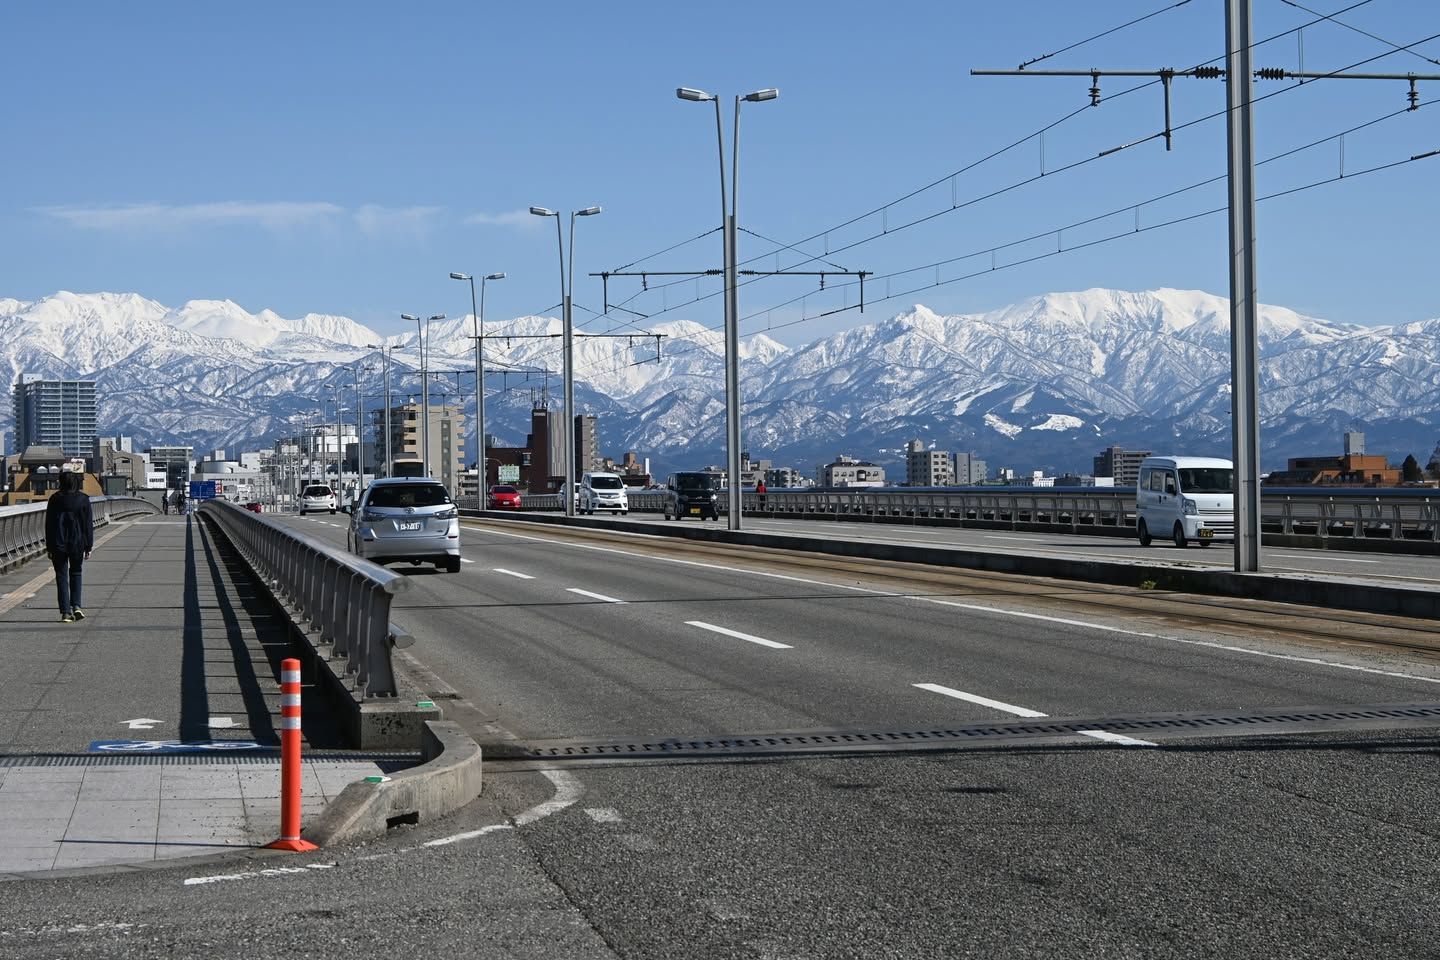
\includegraphics[width=\linewidth]{pictures/2023/02/20230228_223358_001.jpg}
\end{minipage}
\end{center}

\section{3月}

\subsection*{2023年03月03日 18:33}
\addcontentsline{toc}{subsection}{2023年03月03日 18:33}

自宅の梅の木です。

蕾が膨らみかけています。

\paragraph{写真}
\begin{center}
\begin{minipage}{0.70\linewidth}
\centering
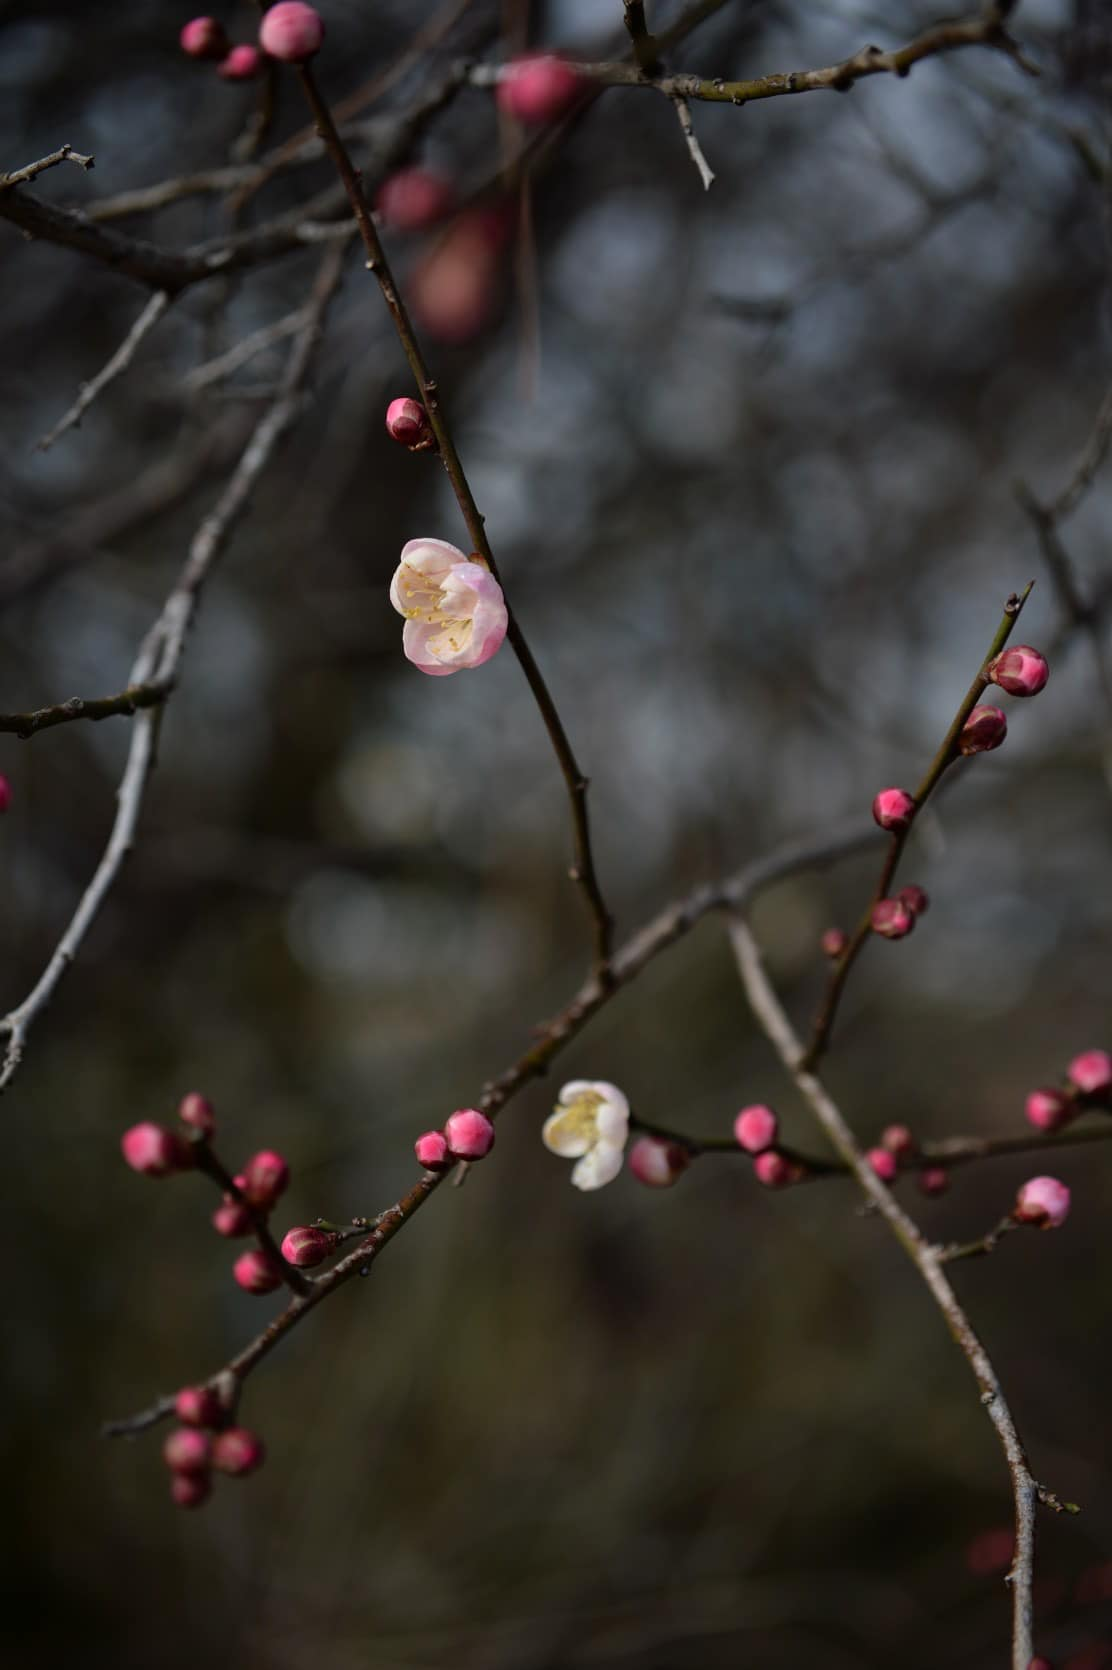
\includegraphics[width=\linewidth]{pictures/2023/03/20230303_183329_001.jpg}
\end{minipage}
\end{center}

\subsection*{2023年03月07日 20:52}
\addcontentsline{toc}{subsection}{2023年03月07日 20:52}

手持ちレンズの中で最も長いレンズで撮ってみた。

天体望遠鏡ではない普通のズームレンズなので、アップにすると色々甘い点が露呈するが、画像編集ソフトでコントラストを上げて、遠目で（小さい画像で）見ていればそれらしく見える。

\paragraph{写真}
\begin{center}
\begin{minipage}{0.70\linewidth}
\centering
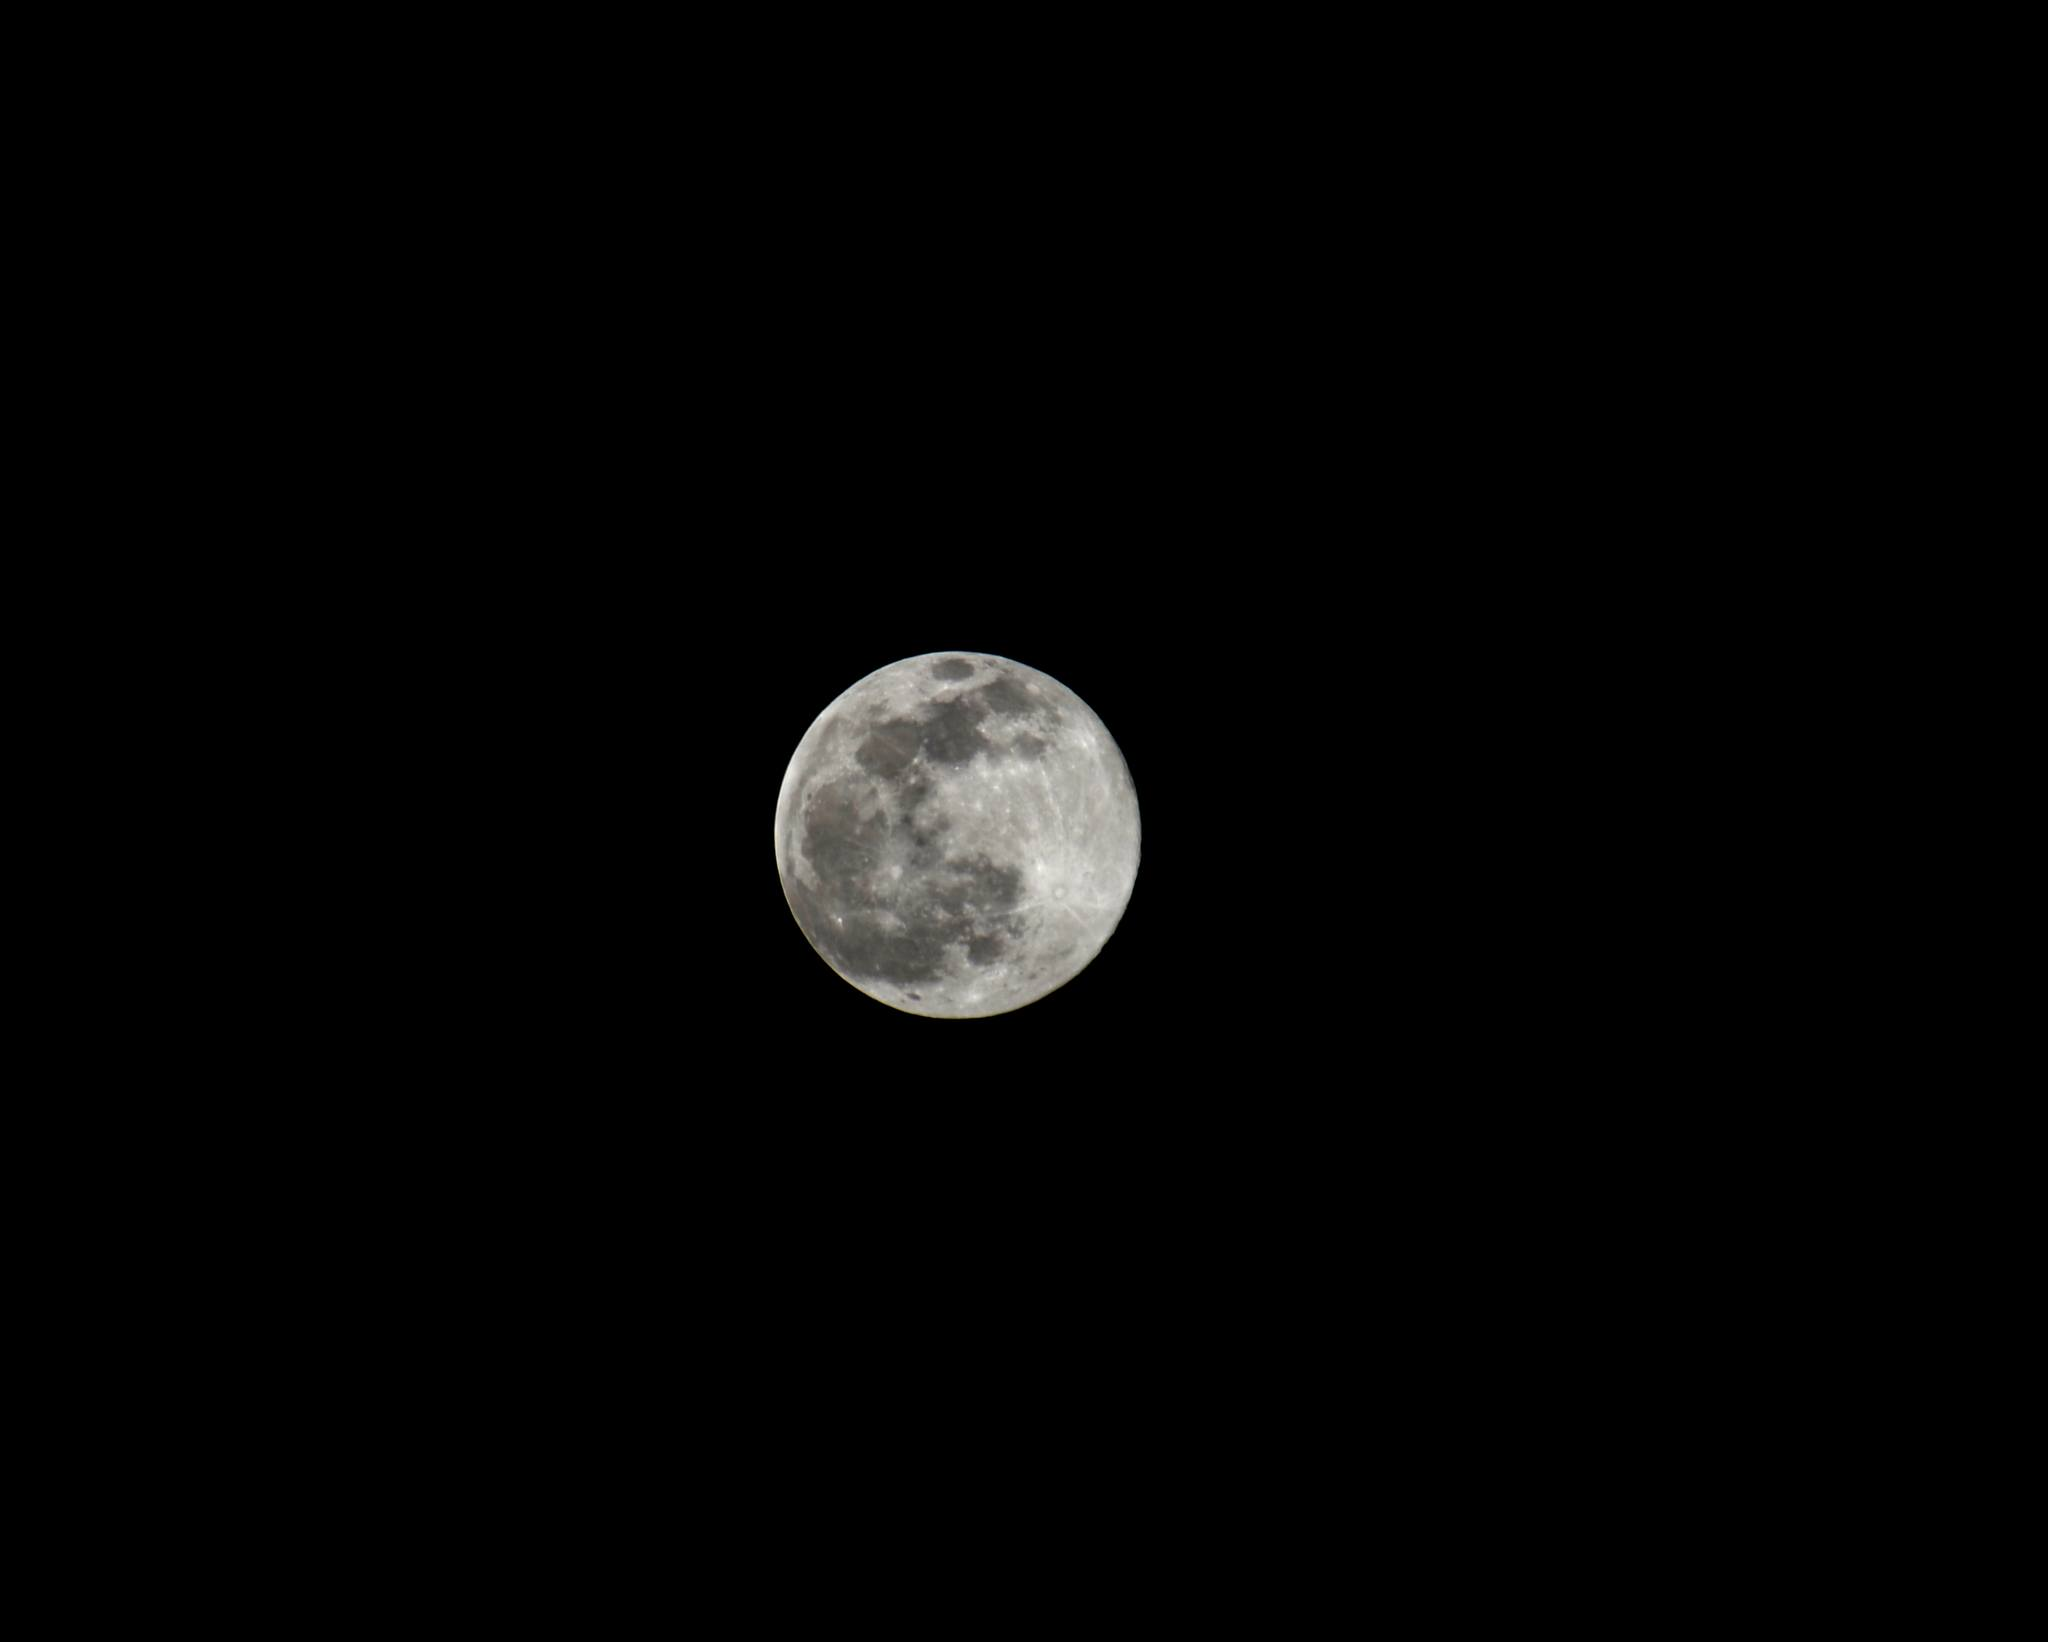
\includegraphics[width=\linewidth]{pictures/2023/03/20230307_205245_001.jpg}
\end{minipage}
\end{center}

\section{4月}

\subsection*{2023年04月10日 08:15}
\addcontentsline{toc}{subsection}{2023年04月10日 08:15}

京都の烏丸通りに面したビルの壁面を見たとき、なんだか見たことある様な気がしました。どうですか、この紋様に見覚えありませんか？

\paragraph{写真}
\begin{center}
\begin{minipage}{0.70\linewidth}
\centering
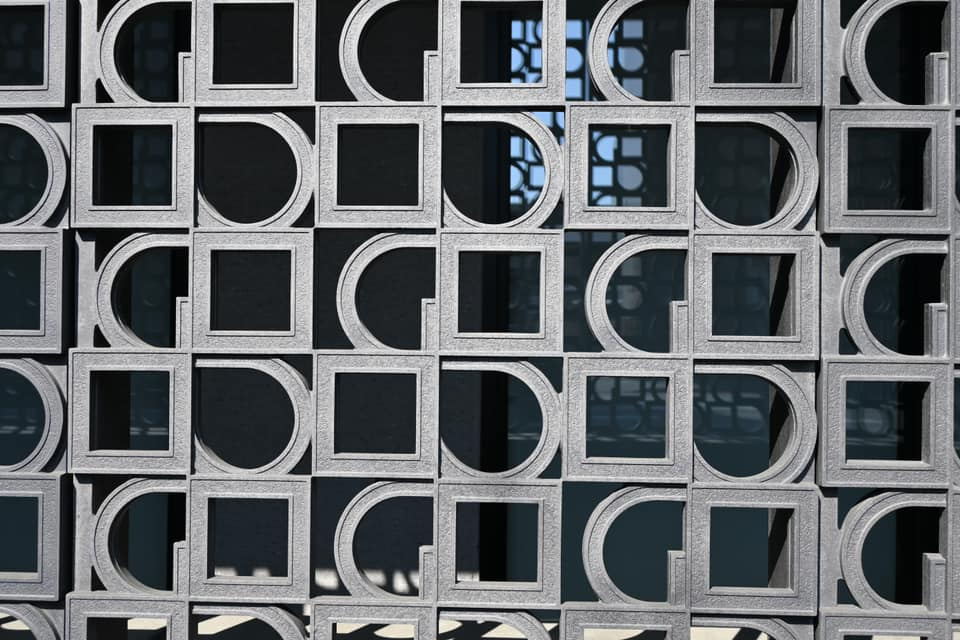
\includegraphics[width=\linewidth]{pictures/2023/04/20230410_081543_001.jpg}
\end{minipage}
\end{center}

\subsection*{2023年04月10日 08:48}
\addcontentsline{toc}{subsection}{2023年04月10日 08:48}

京都の仁和寺(4月9日)です。

桜はもう殆ど散っていましたが、イロハカエデが花？をいっぱいつけていました。また、(弘法大師)空海「自筆」の文書が公開されていました。(国費で派遣された遣唐使エリートの最澄に対して)遣唐使に随行する立場で渡航した空海が現地で密教を学び、記録してきた文書です。私には書いてある内容は読めませんが、とても緻密で綺麗な漢字の書で、その密度の高い漢字の羅列を見ると、全てを記録して持ち帰りたいという空海の強い意志を感じました。こうして中国の文化が伝えられて来たんだなと思います。空海や最澄以外にも、たくさんの遣唐使が日本に伝えようと記録していたのだろうけど、多くは嵐などで海の底に沈んでしまったのかもしれません。(また、中には中国まで辿り着けずに海に沈んでいった人たちも。。)

\paragraph{写真}
\begin{center}
\begin{minipage}{0.70\linewidth}
\centering
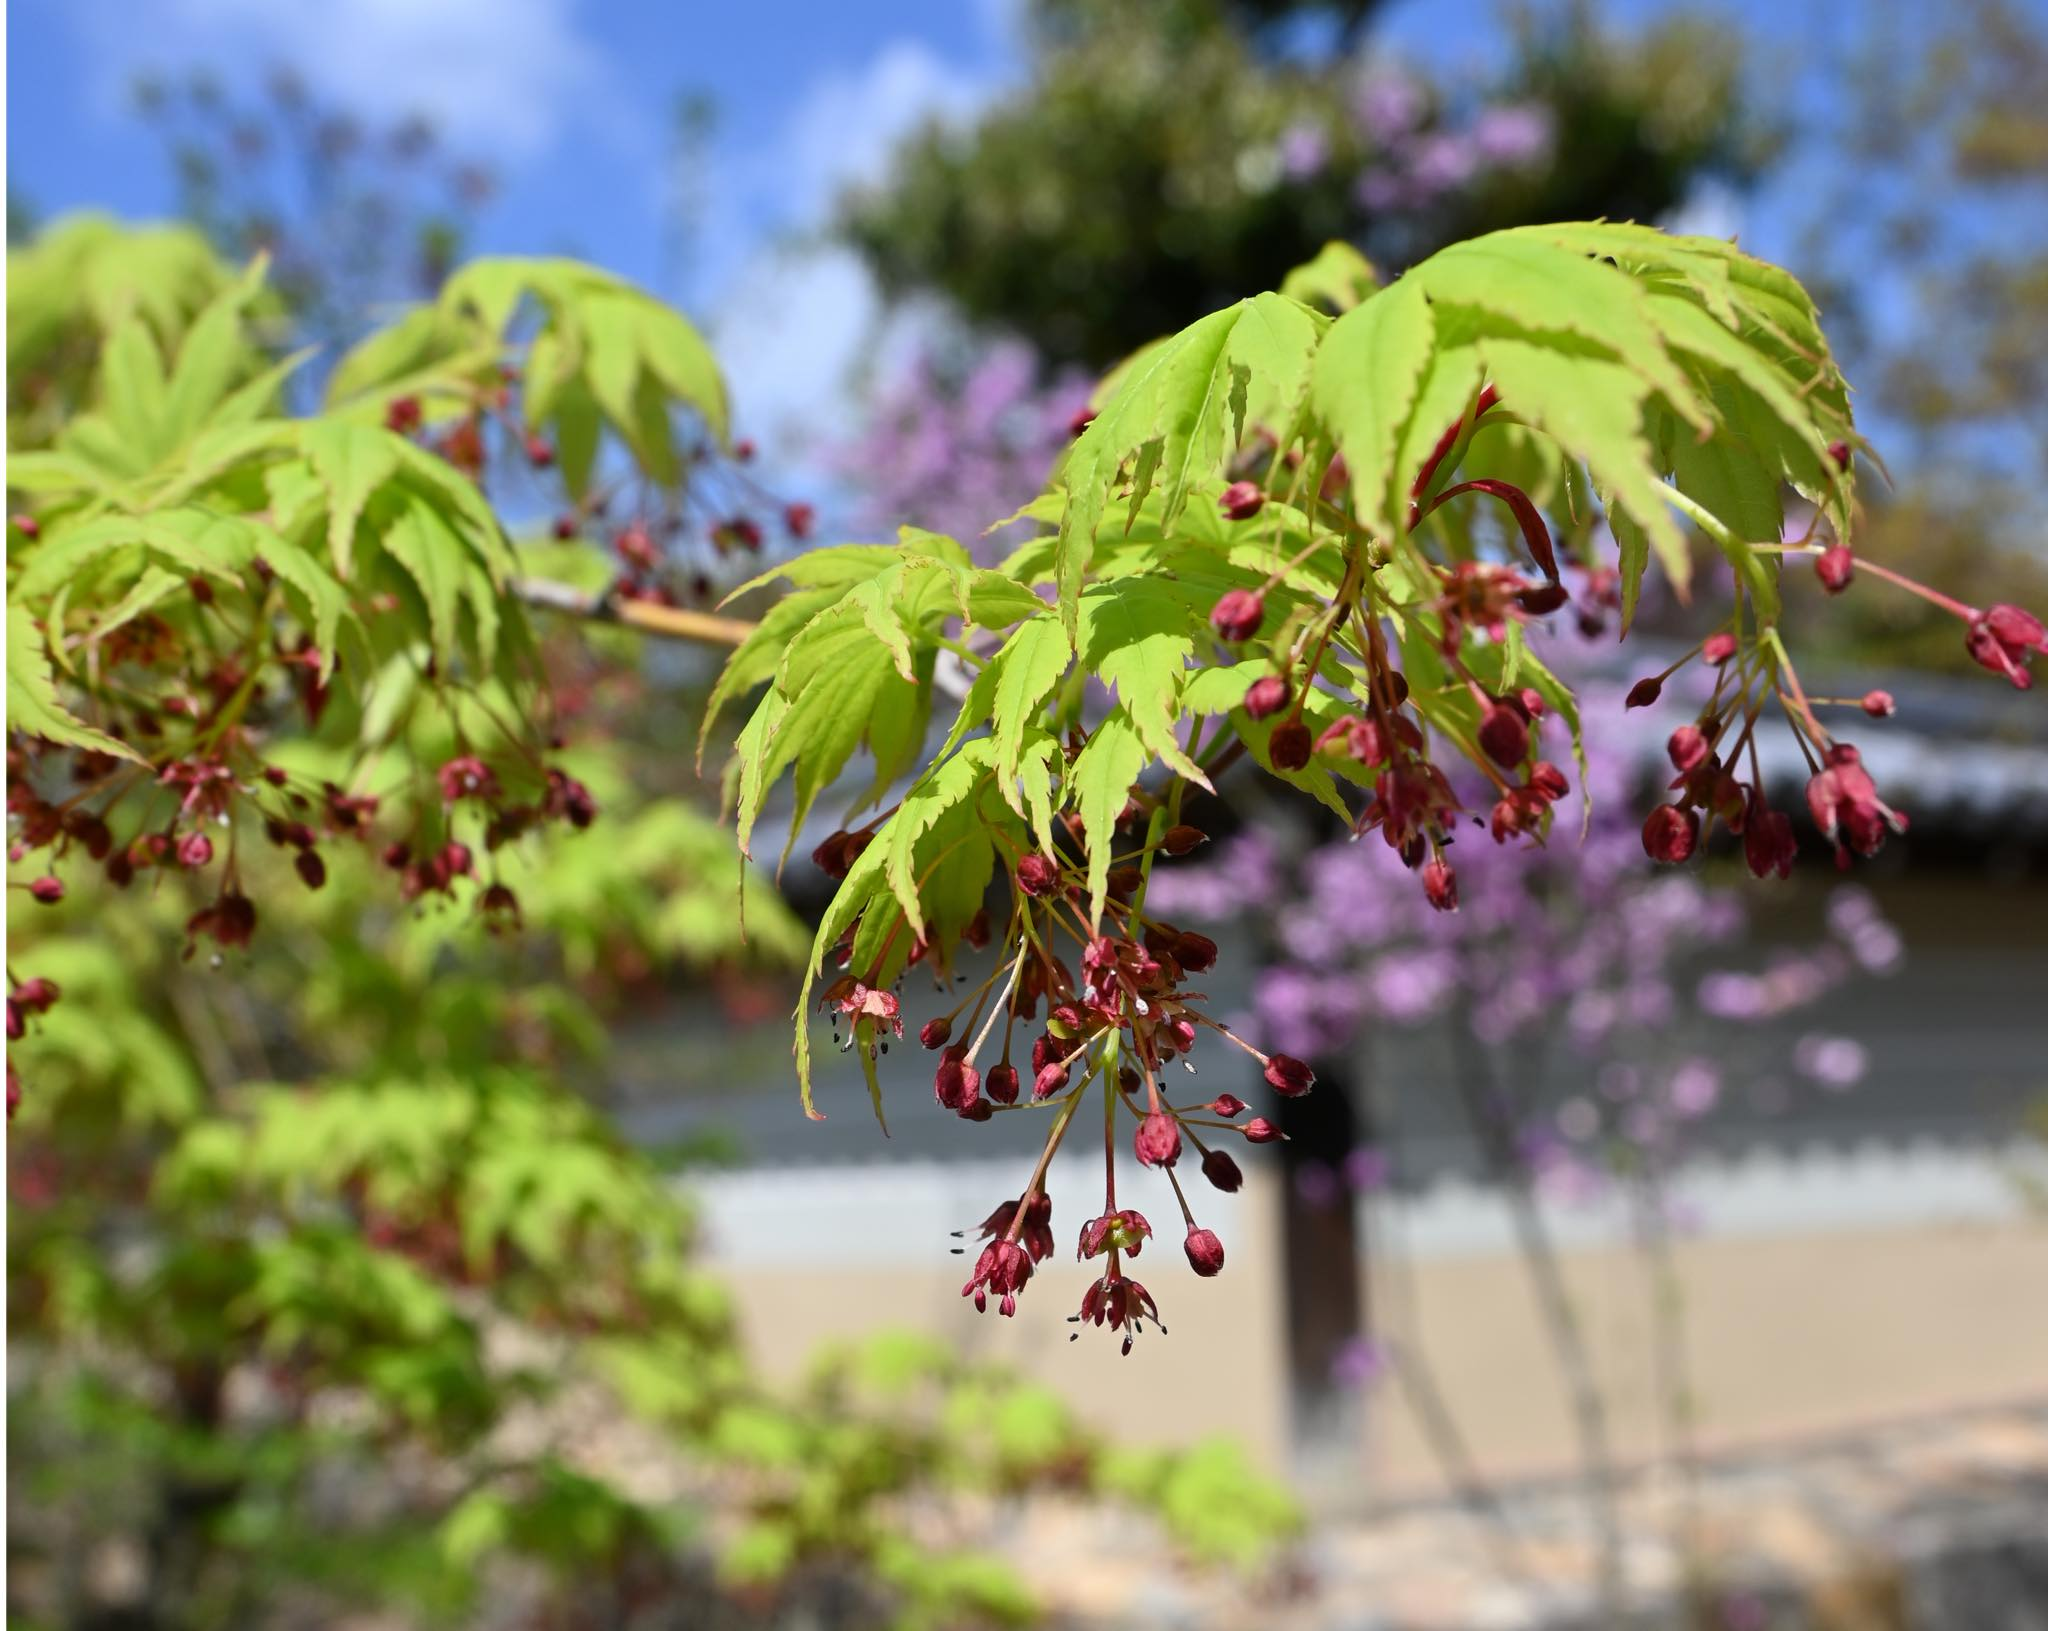
\includegraphics[width=\linewidth]{pictures/2023/04/20230410_084814_001.jpg}
\end{minipage}
\end{center}

\subsection*{2023年04月22日 23:01}
\addcontentsline{toc}{subsection}{2023年04月22日 23:01}

庭の花が先日から気になっていたので撮ってみた。

風で揺れてしまって、被写界深度を深く（＝絞りを絞る＝シャッター速度が遅くなる）できません。たくさんシャッターを押してみました。ブレてないものがあったのでよかった。牧野富太郎氏の図鑑でも見てみようかな。

\paragraph{写真}
\begin{center}
\begin{minipage}{0.48\linewidth}
\centering
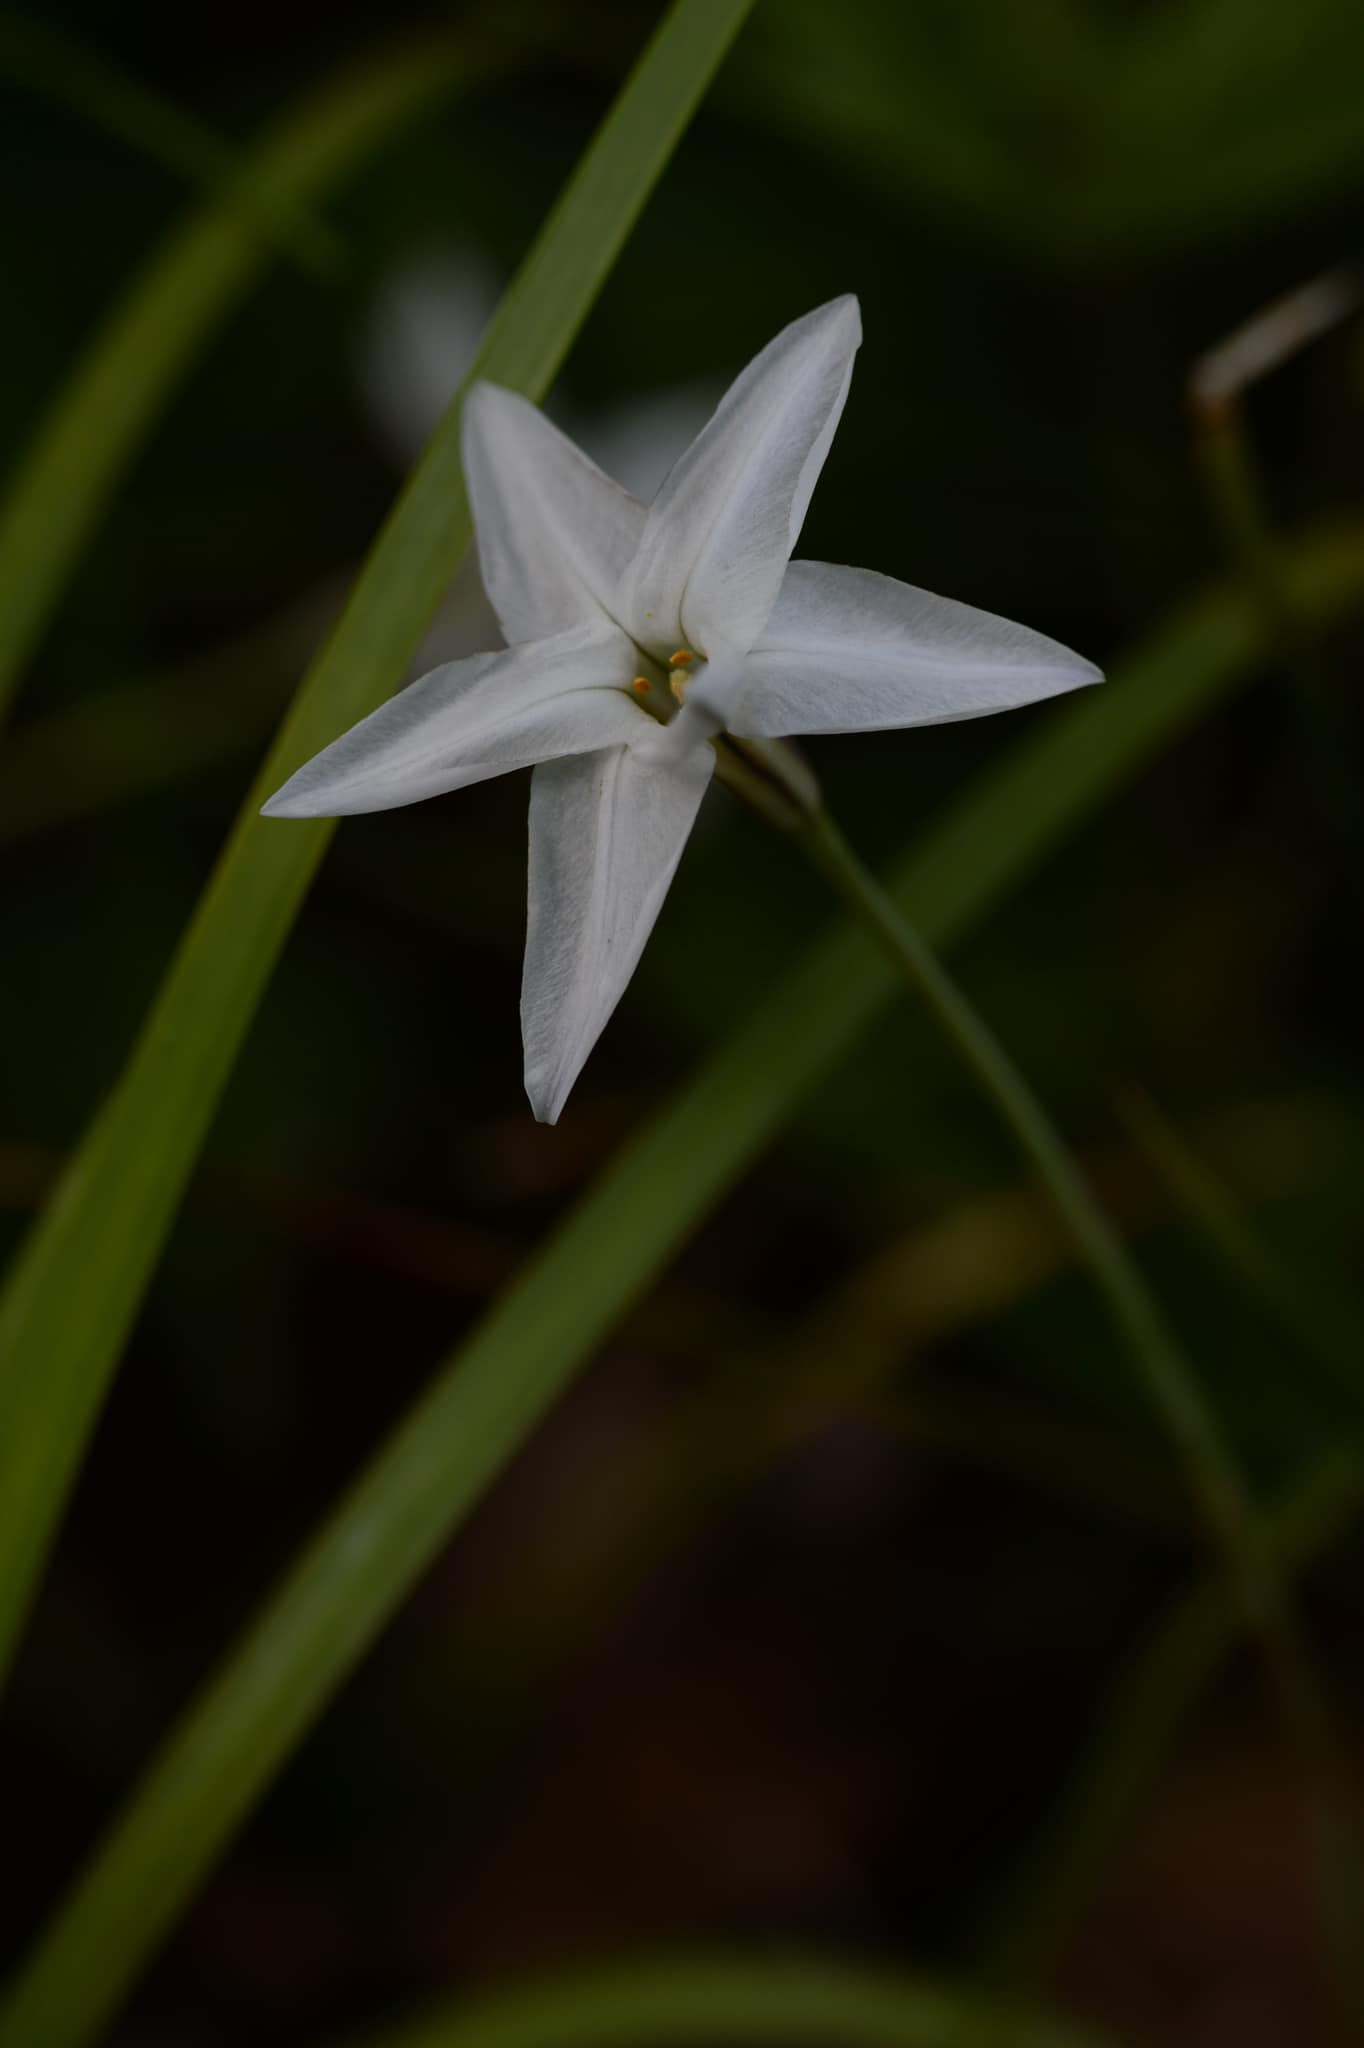
\includegraphics[width=\linewidth]{pictures/2023/04/20230422_230151_001.jpg}
\end{minipage}
\hfill
\begin{minipage}{0.48\linewidth}
\centering
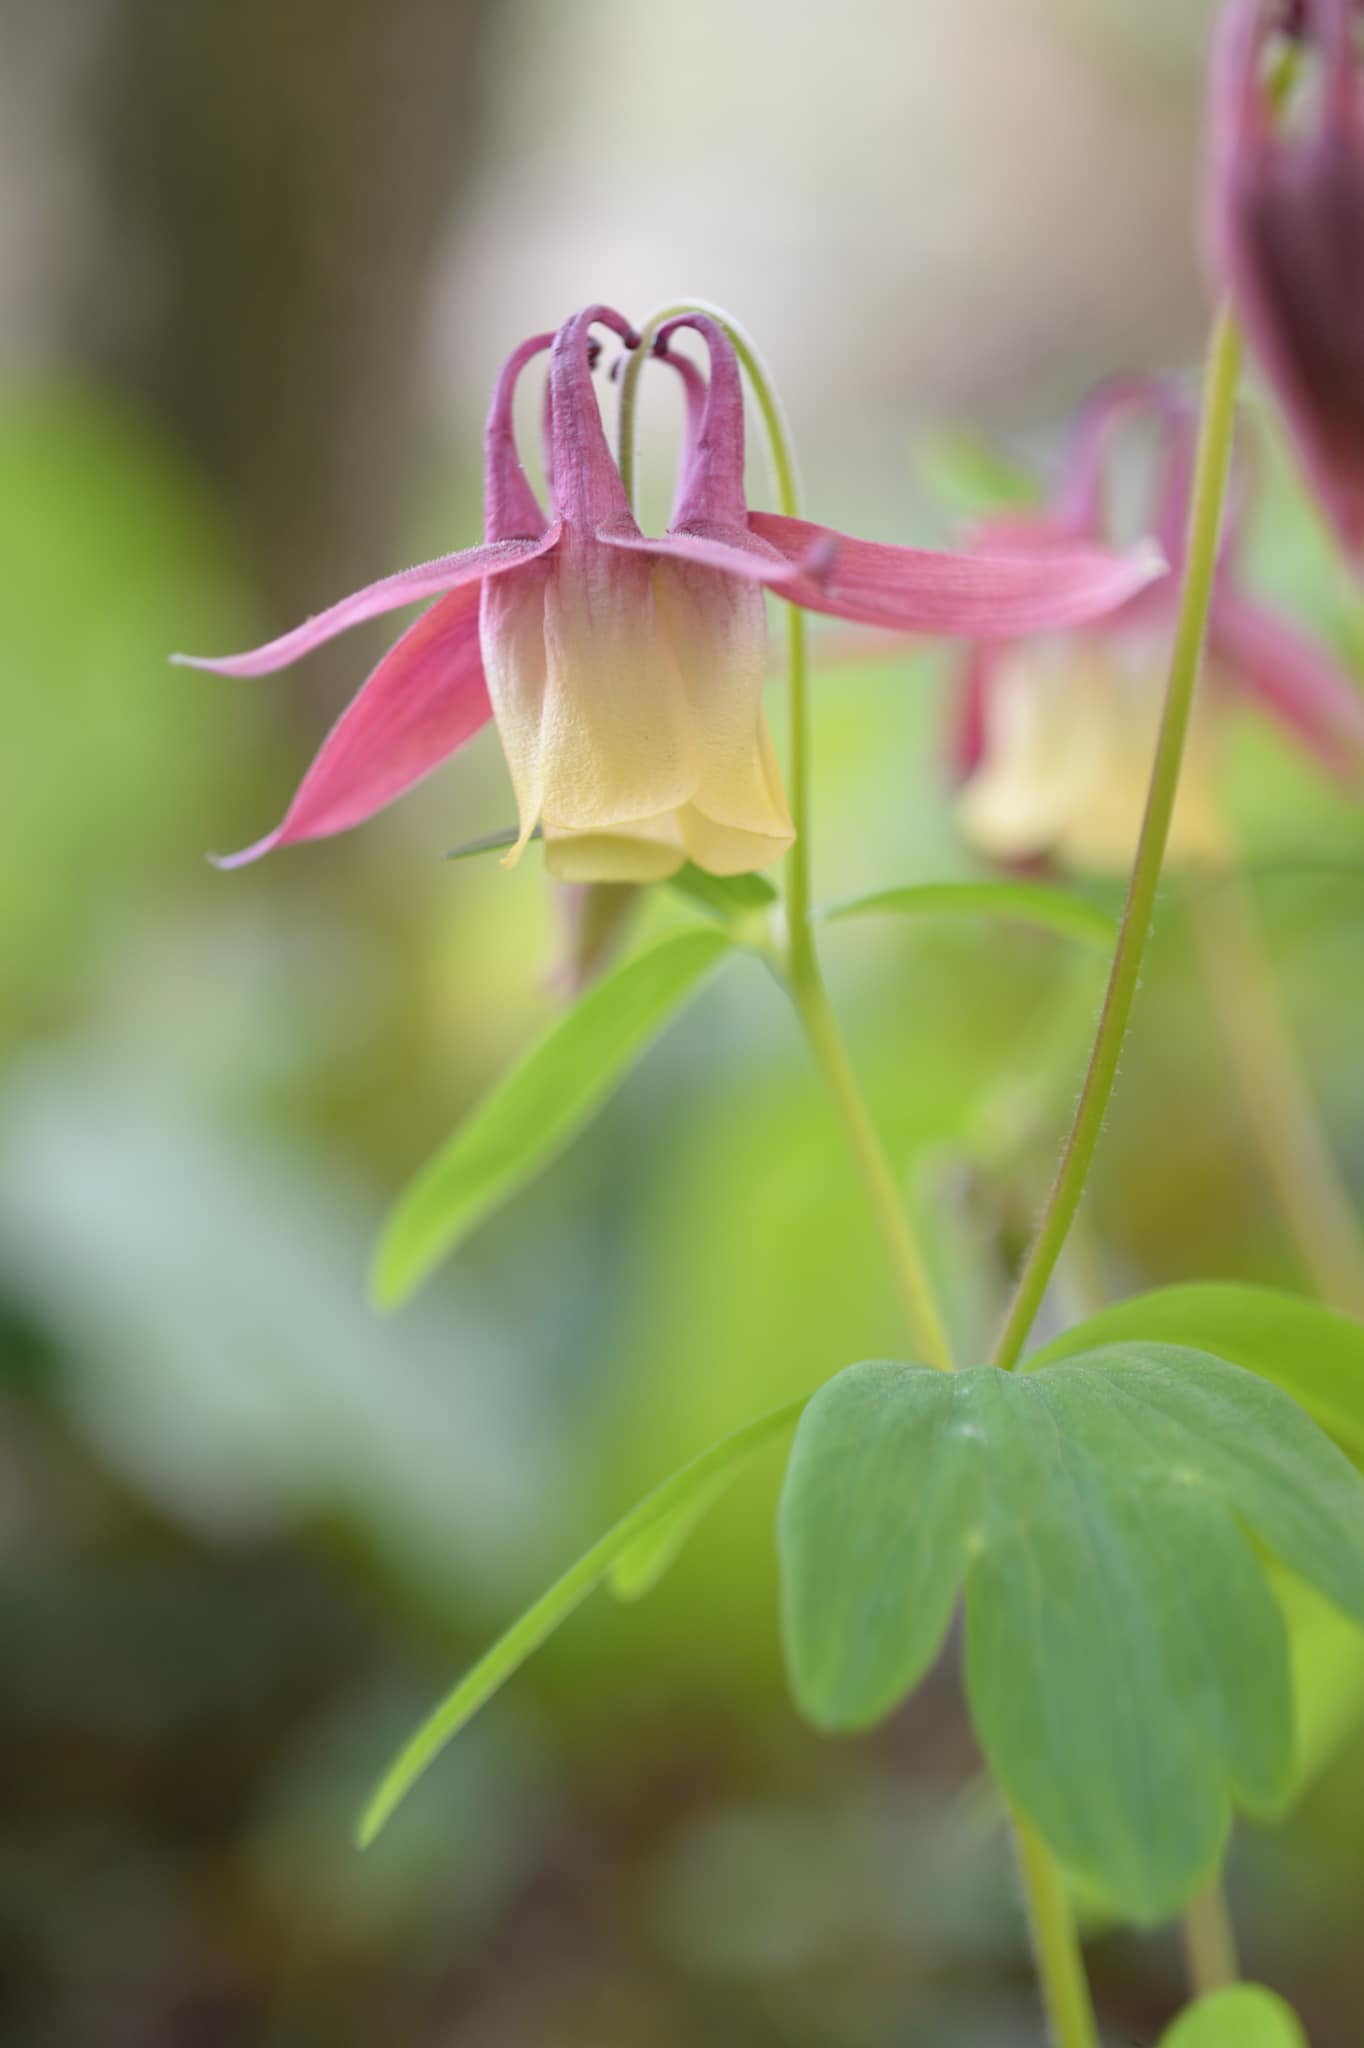
\includegraphics[width=\linewidth]{pictures/2023/04/20230422_230151_002.jpg}
\end{minipage}
\hfill
\end{center}

\section{6月}

\subsection*{2023年06月09日 16:37}
\addcontentsline{toc}{subsection}{2023年06月09日 16:37}

2学期から始まるトランジスタの特性を調べる実習（工業高校2年生）のために、教材になるかもと思って作ってみた。静特性測定用と、周波数特性測定用です。

実際に2SC1815で測定してみると、教科書に出てくるような整ったグラフになるデータがとれて満足です。（測定データからグラフを作図する所ではPythonでプログラムを書いています。本当にPythonは便利ですね。）

製作するにあたっては3Dプリンタが大活躍してくれていますが、特に3Dプリンタでの2色印刷の方法を確立できたことは、個人的に嬉しい点です。また手前の橙色の棒は、実験で可変抵抗器を調整する際に必要になるマイナスドライバですが、これも3Dプリンタで出力したものなんですよ。

\#transistor \#2SC1815 \#特性 \#3Dプリンタ \#Python

\paragraph{写真}
\begin{center}
\begin{minipage}{0.48\linewidth}
\centering
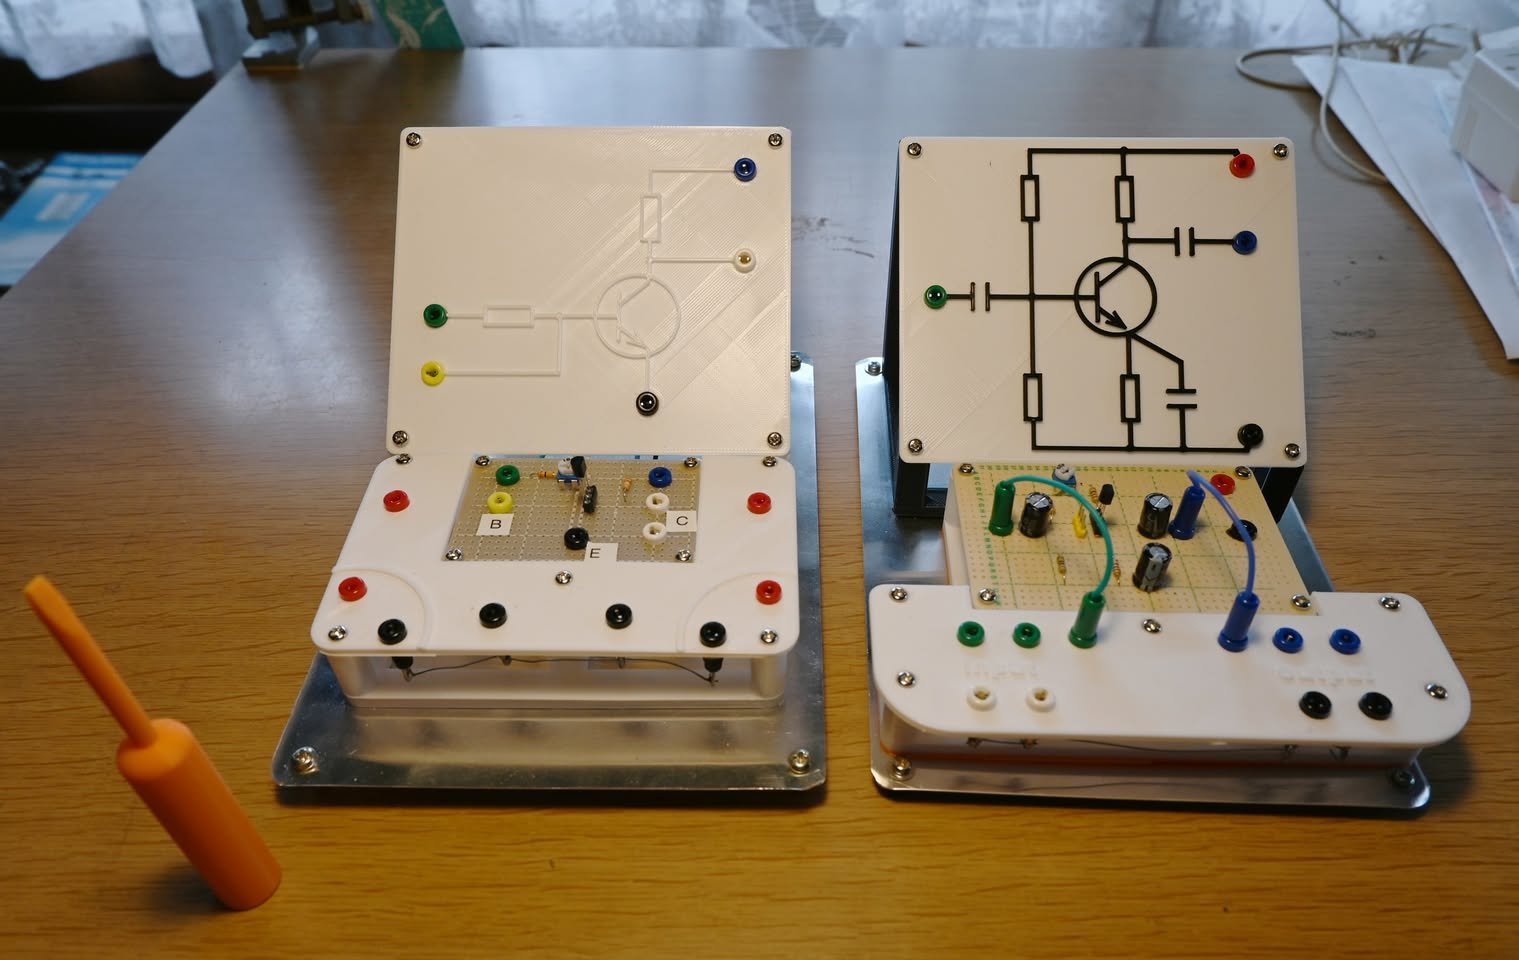
\includegraphics[width=\linewidth]{pictures/2023/06/20230609_163737_001.jpg}
\end{minipage}
\hfill
\begin{minipage}{0.48\linewidth}
\centering
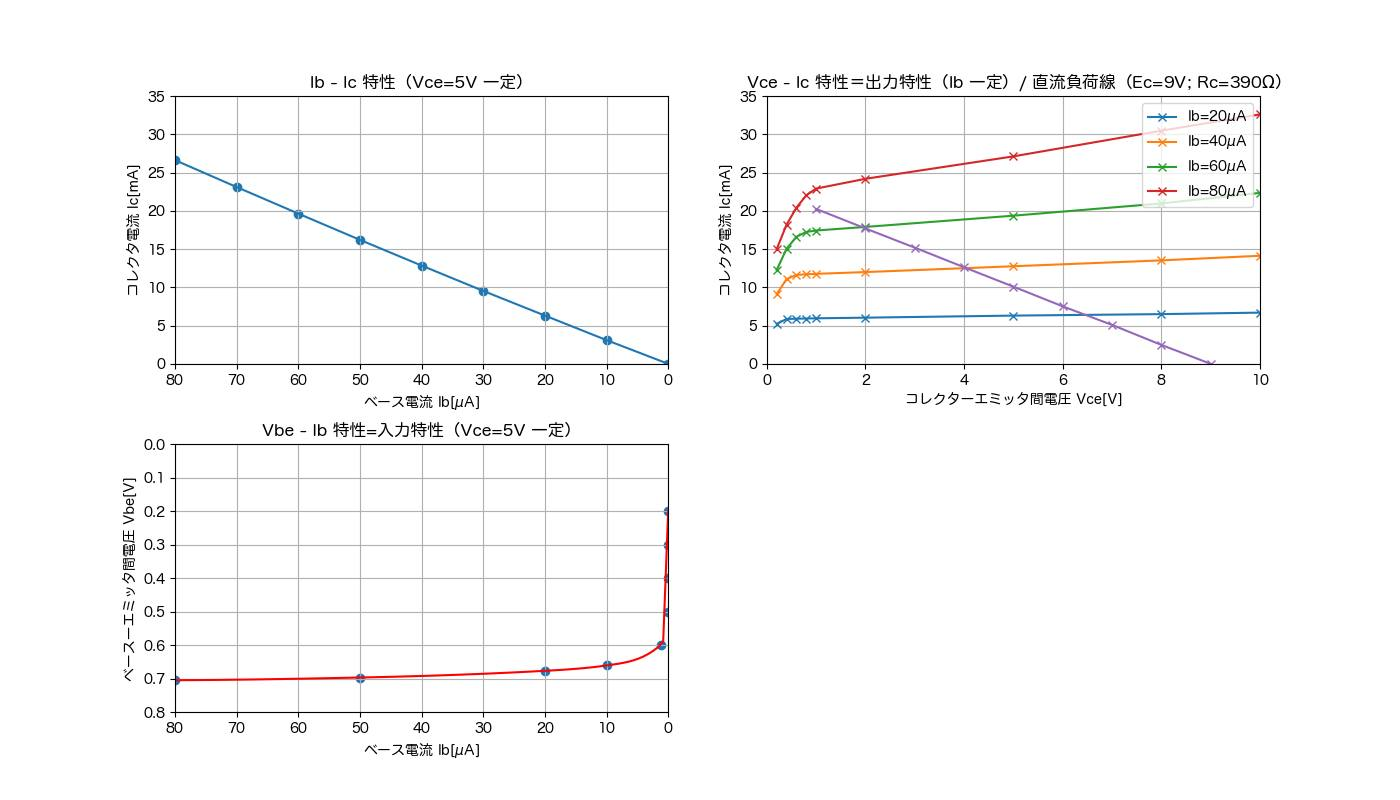
\includegraphics[width=\linewidth]{pictures/2023/06/20230609_163737_002.jpg}
\end{minipage}
\hfill
\end{center}

\begin{center}
\begin{minipage}{0.70\linewidth}
\centering
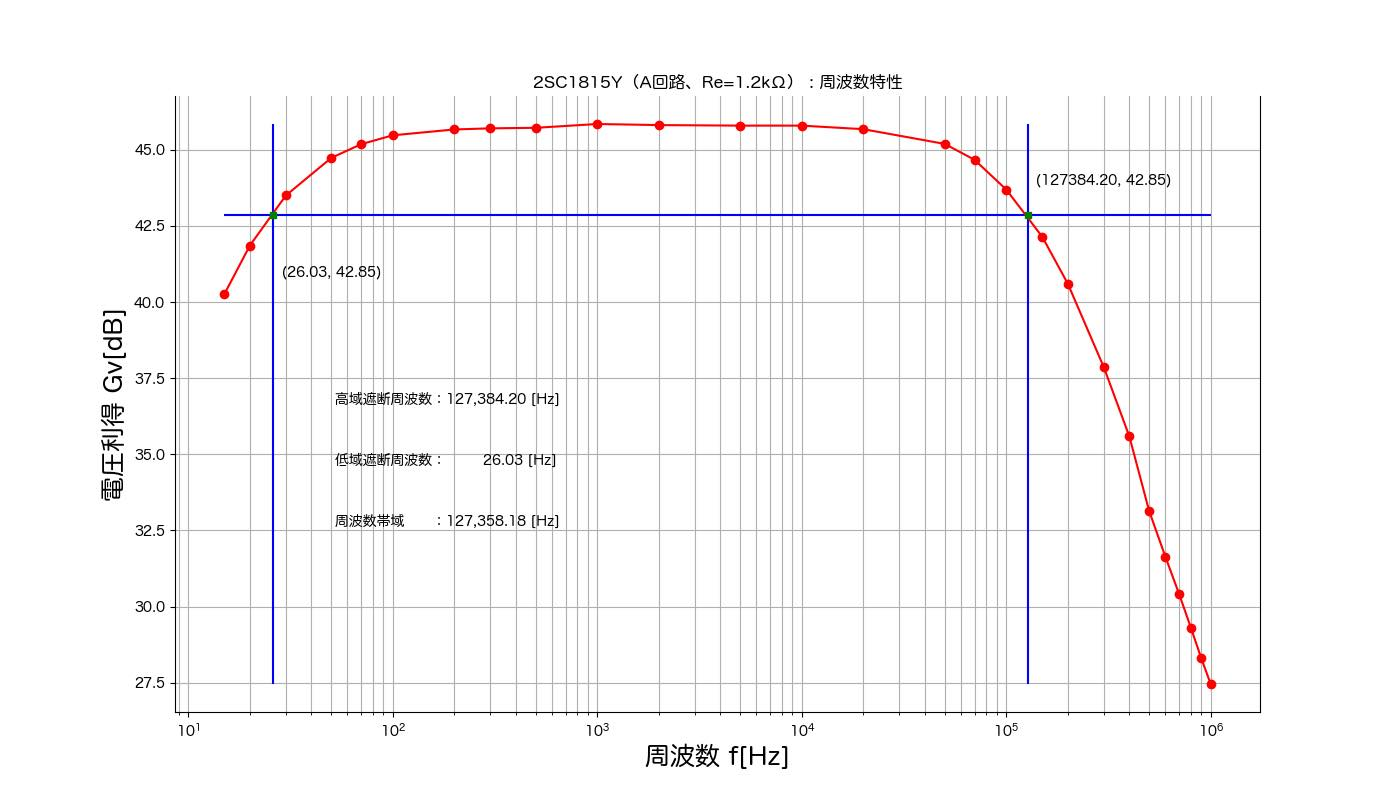
\includegraphics[width=\linewidth]{pictures/2023/06/20230609_163737_003.jpg}
\end{minipage}
\end{center}

\section{7月}

\subsection*{2023年07月25日 06:36}
\addcontentsline{toc}{subsection}{2023年07月25日 06:36}

「アンサンブル音楽三昧」だけど、面白い！

今、ラヴェルのCD -ピアノ協奏曲(の編曲)を聞いている（2楽章はワルツ好きなラベルの真骨頂か？素敵です）んだけど、そもそもオーケストレーションの神様であるとの誉高いラヴェルの曲を、畏れ多くも更に編曲して演奏して（しかも新たな存在、価値を主張、追求して）いると言う代物です。

そもそもが、元々のラヴェルの曲自身が「予想を外したアーティキュレーション」、「訳の分からない響き」、「訳分からん楽器の組み合わせ」だという風に、訳分からん魅力に満ち満ちているのだが、それが更に際立って、ラヴェルって本当に何考えてんのか訳の分からん「すご〜い」人だったんだなとつくづく思います。

凡人に過ぎない私には訳わからんので、面白いとか、すご〜いとか、綺麗とか、訳わからんとかという、言わば凡人にありがちな言葉でしか言い表せません。

\paragraph{リンク}
\url{http://www.cre-a-tion.com/zammai/disco/}

\subsection*{2023年07月25日 11:10}
\addcontentsline{toc}{subsection}{2023年07月25日 11:10}

「Effective Python」は良い。

最初から順に読む必要はない。目から鱗の情報が随所に書かれている。

そもそも、この「Effective何某」という本に出会った最初の出来事といえば、昔々（もう30年近く昔のことではなかったか？）「Effective C++」という本に出会ったことです。自分のプログラムの書き方に非常に大きな影響を受けたという記憶があります。その後「Effective Java」とか、あったのか無かったのか調べていないけれど、今回Pythonで再び出会うことができたという感じです。そう「Effective C++」の時もこんな感じだったかな。

そういえば本書の初めの所で「他の言語に馴染んできたプログラマは、Pythonをあたかも、C++やJavaと同じであるかの様に書こうとする」と書かれています。耳の痛い指摘ですね。Pythonicな書き方を身につけるには、この本はベストな選択肢になるように思います。

\paragraph{リンク}
\url{https://www.oreilly.co.jp/books/9784873119175/}

\subsection*{2023年07月25日 23:19}
\addcontentsline{toc}{subsection}{2023年07月25日 23:19}

「トランジスタ実習（工業高校2年生）」のための実習テキストを書いてみた。一応それなりに事前の実験をしています。実習に使う実験回路の製作及び実際の事前実験では、座学で使っている教科書「電子回路」（実教）を参考にしています。

テキストは、以下のGitHubのリンクから。

src/out/transistor.pdfは事前実験の内容をまとめています。

src/out/practice.pdfは実習の際に配布予定の実習テキストです。

src直下には、各PDFを作った時のTeXのソースも置いています。

\#transistor \#特性 \#GitHub \#Python \#VSCode \#TeX \#illustrator \#rigol \#LTspice

\paragraph{リンク}
\url{https://github.com/smat1957/transistor_practice}

\section{8月}

\subsection*{2023年08月08日 21:21}
\addcontentsline{toc}{subsection}{2023年08月08日 21:21}

\#こまつ座「\#闇に咲く花」

今ほど、新宿のTAKASHIMAYA で観てきた所です。

井上麻矢氏がパンフの巻頭言で、ウクライナの戦争や宗教のあり方等に触れて「これほどにこの作品が上演されるのが相応しい時期はない」とコメントされています。原作者井上ひさし氏のメッセージ「忘れ（たふりをし）てはいけない」。栗山民也氏の演出、山西惇氏をはじめとする皆さんの熱い演じ、そしてギター弾きの水村直也氏による生クラシックギターの素朴な音の響き（ラグリマ、アストーリアスの片鱗等）、これこそ（総合）芸術をマノアタリにしたという印象です。

最後のシーン、靖国神社の太鼓が地響きのように繰り返し鳴る不気味な音は、忍び寄る軍拡への歩みを連想させます。その音に恐れ慄いて身を寄せ合う庶民の姿。このラストシーンは、演出家による強いメッセージ（「忘れてはいけない」を言い続けても忘れてしまう。それでも言い続けなければならない。）と受けとめました。私も含めて、大衆（=花、軍拡のどす黒い雲の下=闇、に咲いている）とは、忘れやすい人種なんだと思う。よもやもう一度、大規模な人殺し（=戦争）をやらされなければ思い出せないとでも？……不毛であることに、やり場のない怒りを覚えると共に、悲しくなります。

原作者が亡くなられても、作品はこうして上演されて、主張し、警鐘を鳴らしながら、残っていくのですね。

⚪︎8月4日から30日まで東京・紀伊國屋サザンシアター TAKASHIMAYA

⚪︎9月2・3日に愛知・東海市芸術劇場 大ホール

⚪︎6日から10日まで大阪府 新歌舞伎座

⚪︎12・13日に福岡・キャナルシティ劇場

\paragraph{写真}
\begin{center}
\begin{minipage}{0.70\linewidth}
\centering
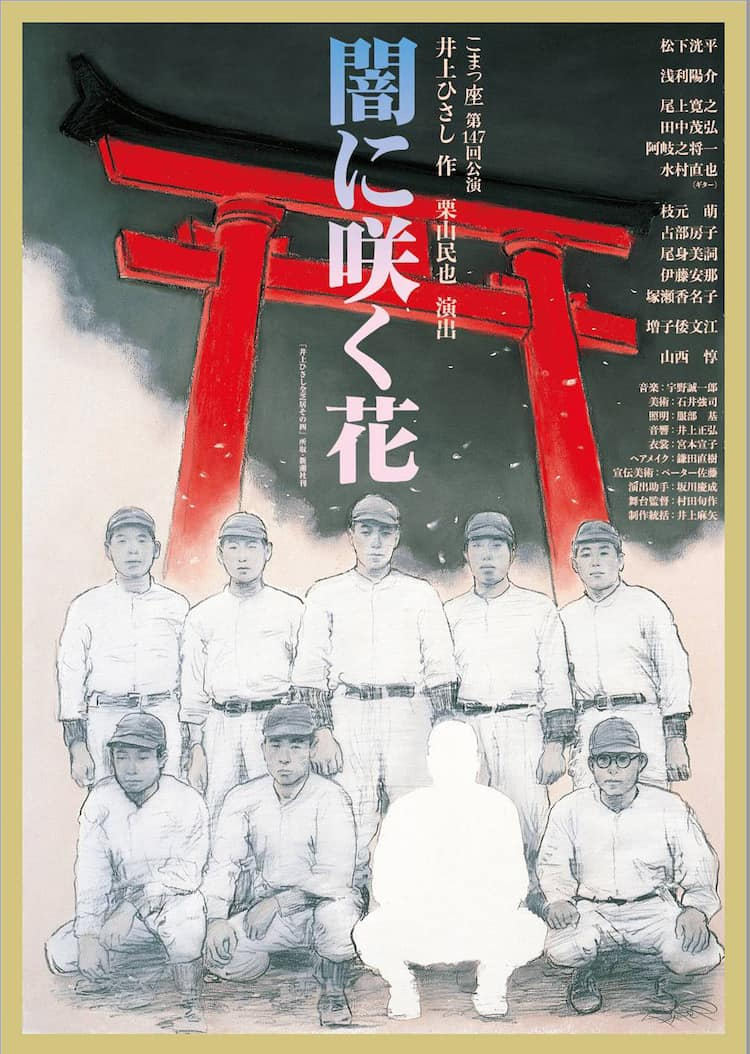
\includegraphics[width=\linewidth]{pictures/2023/08/20230808_212119_001.jpg}
\end{minipage}
\end{center}

\subsection*{2023年08月31日 23:26}
\addcontentsline{toc}{subsection}{2023年08月31日 23:26}

Mac対応のVSCodeが、一年後に終了するらしい。

エディタは日常使いの文房具ですから、人によって好みがあると思います。

MicrosoftのOfficeは、お仕事が現役だった頃にはそれなりにお世話になりましたが、subscriptionになったのでUninstallして、pages、numbers、keynoteで代用することにしました。そしてVSCodeですが、だんだん機能てんこ盛りのゴリゴリになってきたと感じていました。この機会にUnInstallすることにしました。

MacにはTeXShopというTeX文書作成環境があります。VSCodeでTeXを書いていて、TeXがエラーで止まったりする時に、どこが原因なのか分からなくなる事があります。そんな時、同じソースをTeXShopにかけてエラー箇所を見つけるという使い方をしていました。TeXShopは緊急時のために担保しておくことにして、それとは別にVSCodeに代わる環境を探しているのです。

VSCode以前には、AtomとSkimを連携させてTeX用に使っていました。AtomはTeXエディタとしてそれなりに快適でしたので、TeXShopの出番もなかったのですが、新たな開発サポートをやらなくなってしまったので、渋々VSCodeに移住してきたのでした。今更、ネットに転がっているAtomの旧バージョンを探してきてinstallする気にもなれません。また、viエディタやEmacsを使っていた時代にまでさかのぼる気力も失せてきているので、あらためてモダンな環境を探すことにしました。

TeXStudioを試してみようと思います。vi、Emacs、Atom、VSCodeは汎用のエディタですが、TeXStudioはTeX専用の文書作成環境です（TeXShopと同様）。これをMacで動かすためには、設定で各種コマンドへのpathを変えてあげなければなりません。誰かMacで動かしている先人がいるはずだと思い、それをネット上で探してきて、今ほど設定を終えた所です。これが気にいるかどうか、しばらく様子を見たいと思います。

\section{9月}

\subsection*{2023年09月04日 03:37}
\addcontentsline{toc}{subsection}{2023年09月04日 03:37}

\#フリードリヒ2世 の \#サンスーシ宮殿 での演奏会の様子が描かれた絵の一部拡大ですけど。いつも絵の全体をPC画面サイズで見るだけで、部分的な詳細を見たのは初めてです。

J.J.Quantz、E.Bach、F.Bendaこんなに表情までクリアに描かれているとは知りませんでした。もともと全体はどんなサイズの絵なんだろう？

\paragraph{写真}
\begin{center}
\begin{minipage}{0.70\linewidth}
\centering
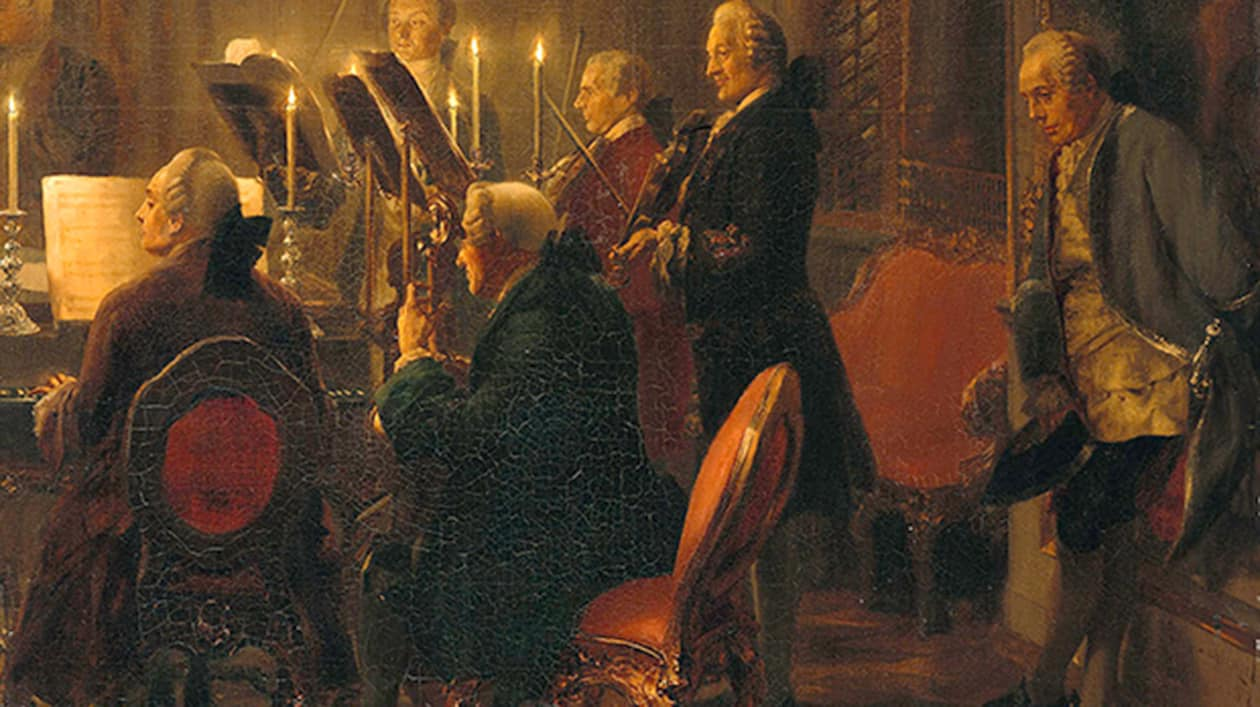
\includegraphics[width=\linewidth]{pictures/2023/09/20230904_033703_001.jpg}
\end{minipage}
\end{center}

\subsection*{2023年09月28日 17:30}
\addcontentsline{toc}{subsection}{2023年09月28日 17:30}

準備してきたトランジスタの実習（工業高校2年生）。

みんな真剣に取り組んでくれました。

丁度、座学での学習項目とタイミングがあっていたらしくて、「0.6Vからベース電流流れはじめた」など、反応がよくてやり甲斐がありました。

\paragraph{写真}
\begin{center}
\begin{minipage}{0.70\linewidth}
\centering
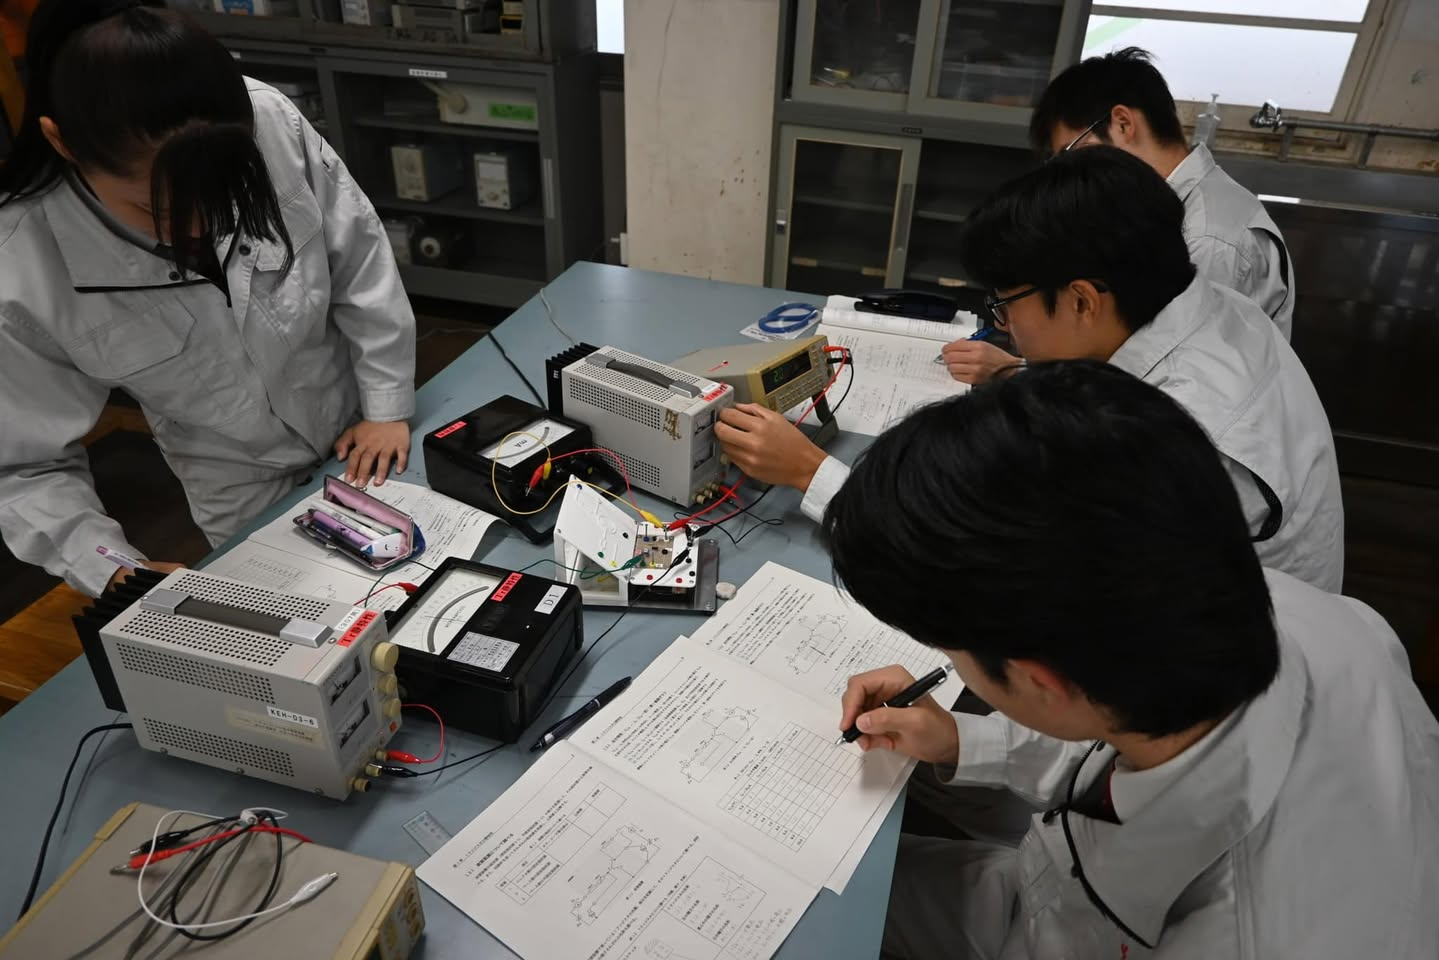
\includegraphics[width=\linewidth]{pictures/2023/09/20230928_173038_001.jpg}
\end{minipage}
\end{center}

\subsection*{2023年09月29日 04:03}
\addcontentsline{toc}{subsection}{2023年09月29日 04:03}

御著書を何冊か積ん読しております。お会いしたこともないですし、従ってお人柄も存じ上げておりません。でも、御著書から、陰ながらそして勝手ながら尊敬させて頂いておりました。朝永振一郎氏による啓蒙書の（いささか専門的な）解説も書いていらっしゃいます。また、培風館から出ていた新物理学シリーズ36の「解析力学」ですが、ちょっと残念な事に誤植？がとても多いです。しかしその点を許容しても尚あまりある、その内容にこそ惹きつけられるものがありました。とても気に入っていたので、改訂版などを期待していたのですが。お悔やみを申し上げます。

\paragraph{リンク}
\url{https://www.sankei.com/article/20230928-Q5F4LFKIJBNSZN37QGPE2SZW5Y/}

\section{10月}

\subsection*{2023年10月06日 10:45}
\addcontentsline{toc}{subsection}{2023年10月06日 10:45}

トランジスタの静特性を測定する実習（工業高校2年生）が、最終の班を迎えるばかりになって、その後に始まる予定の「増幅回路の周波数特性の測定実習」についてふと思いを馳せていると、測定データを整理する際に必要になる片対数のグラフ用紙が、市販のものでは横（周波数）の方向に1デカード(decade)分だけ足りなかったということを思い出した。

2枚のグラフ用紙をハサミで切って、糊で貼り付けて伸ばすことや、真ん中で分けて左側と右側をそれぞれに書いて、2枚1組でレポート提出用にしたら、などと考えたりしていたが、いやいや自前で片対数の \#グラフ用紙 を用意したらいいじゃないかと思うようになった。

添付のように \#Python で \#片対数グラフ 用紙を作図するプログラムを書いてみた。朝思いついて、にわかに書いてみたプログラムなので、スマートじゃないかもしれないけど、とにかくできた。ということで、このグラフ用紙をコピーして配ることにしよう。

\paragraph{写真}
\begin{center}
\begin{minipage}{0.48\linewidth}
\centering
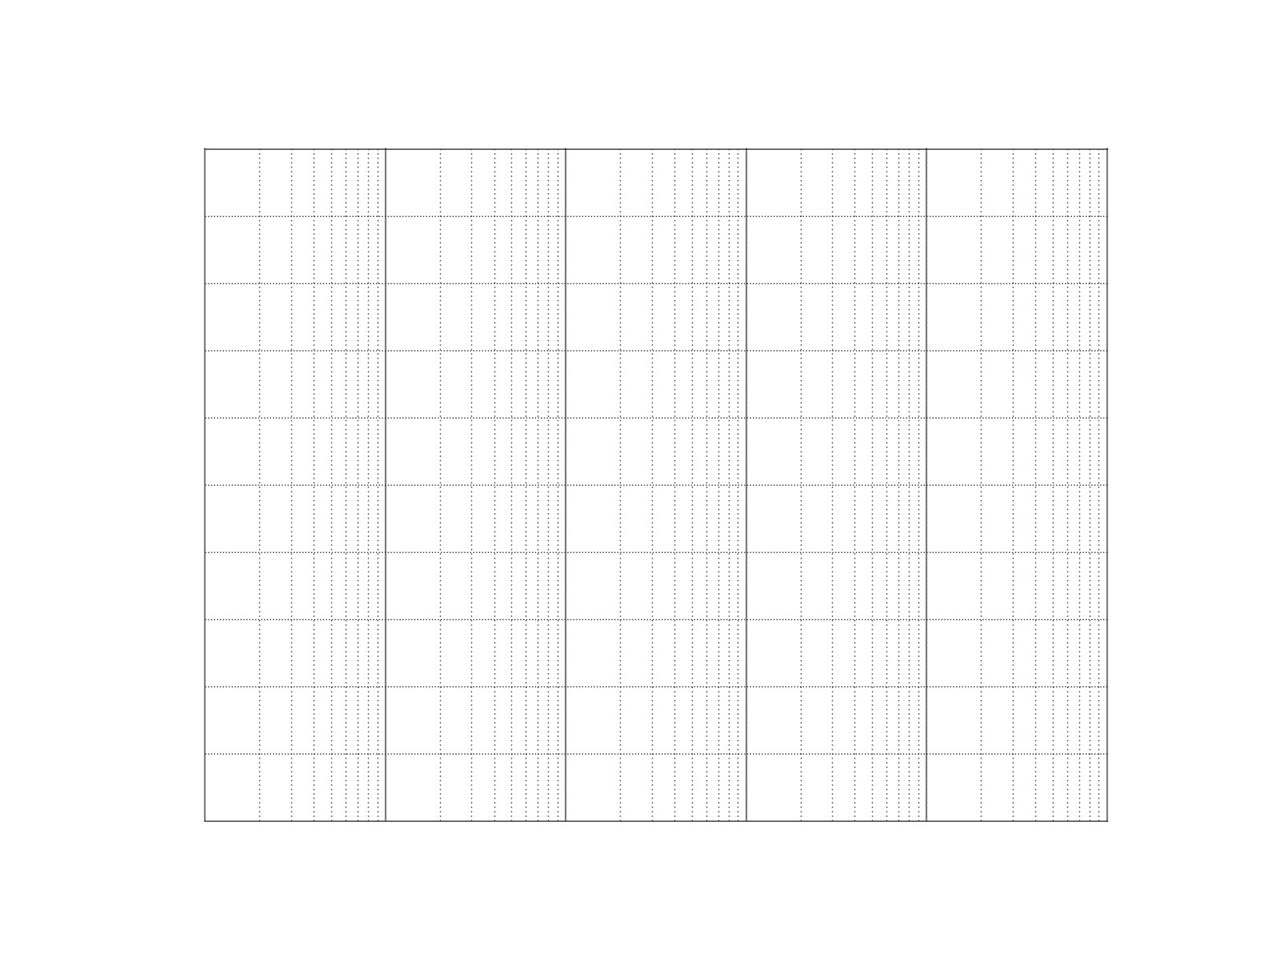
\includegraphics[width=\linewidth]{pictures/2023/10/20231006_104505_001.jpg}
\end{minipage}
\hfill
\begin{minipage}{0.48\linewidth}
\centering
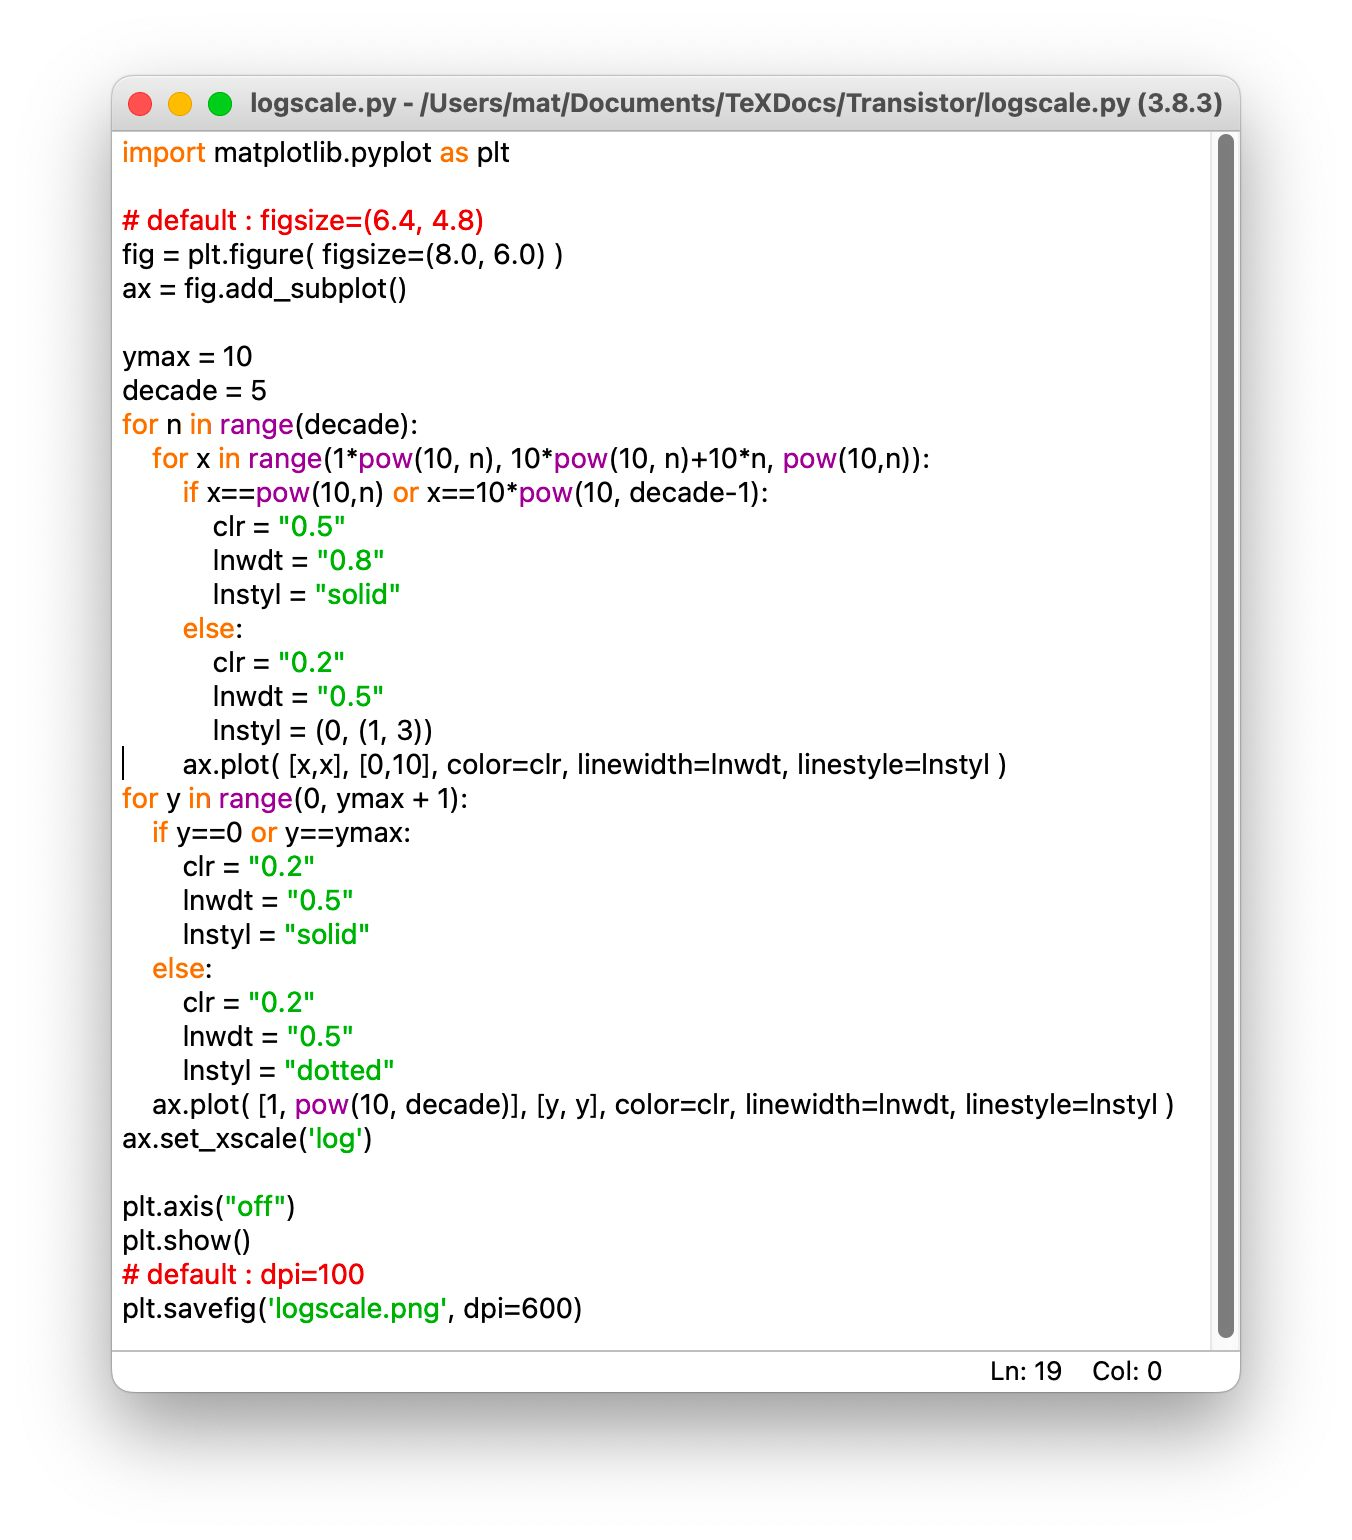
\includegraphics[width=\linewidth]{pictures/2023/10/20231006_104505_002.jpg}
\end{minipage}
\hfill
\end{center}

\subsection*{2023年10月08日 21:53}
\addcontentsline{toc}{subsection}{2023年10月08日 21:53}

\#CUI  による \#オセロ の \#ゲーム をプログラム（ \#C言語 ）してみた。

意識しているのは、「プログラミング技術」という教科書（実教）を使っている工業高校2年生の座学の科目。（この教科書は、最初から最後まで詳しいC言語のテキストブックになっている。）

GUIのゲームにしないのは、GUIに関する（追加の）学習をしなくてもいいから。プログラムを、なるべく短くてシンプルな格好で提示したいからです。Emacs の画面を見ると209行になっている。コメント行を数えなければ200行を切るはず。でも、もうこれ以上スリムにできないな。

JavaにしてもPythonにしても、オブジェクト指向でプログラムする事が普通の世の中になっているので、オセロの様な、この程度の小規模なプログラムでさえ、もはや「オブジェクト指向できないC言語」によるプログラミングというのは少々苦痛に感じてしまいます。先ず最初にどこから手をつけようかと考え込む事になります。mainから書きはじめて、必要になる関数サブプログラムを次々に追加していく感じになるかな。

\paragraph{写真}
\begin{center}
\begin{minipage}{0.70\linewidth}
\centering
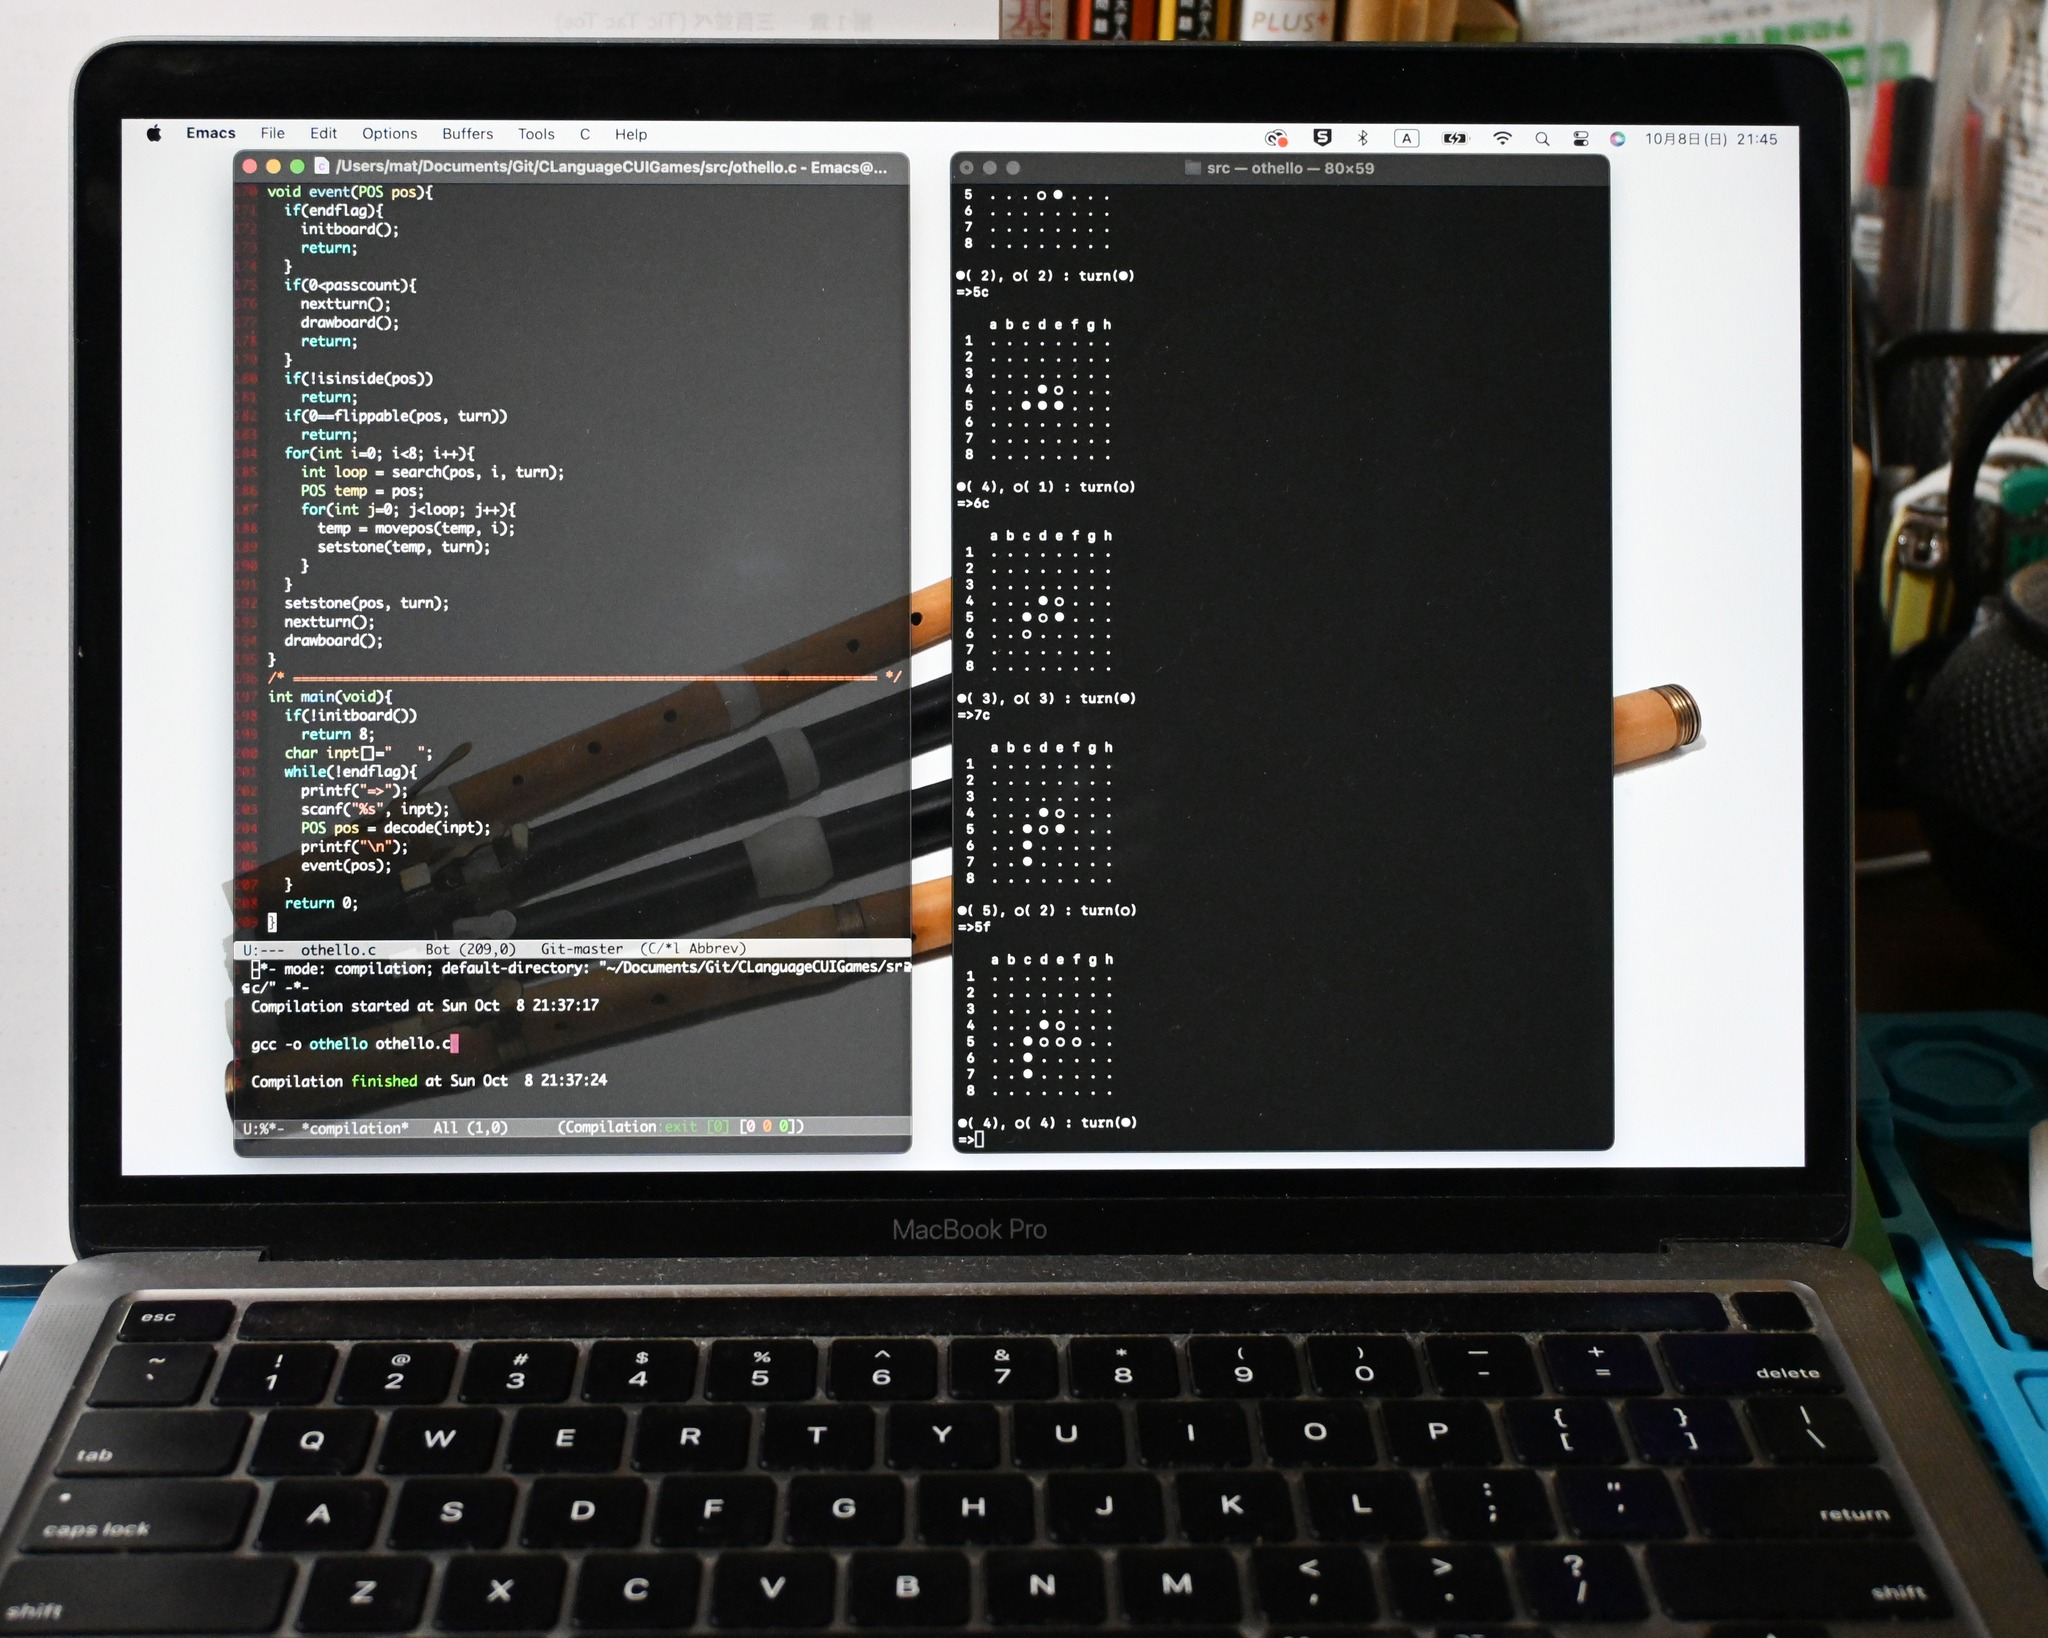
\includegraphics[width=\linewidth]{pictures/2023/10/20231008_215346_001.jpg}
\end{minipage}
\end{center}

\subsection*{2023年10月21日 16:36}
\addcontentsline{toc}{subsection}{2023年10月21日 16:36}

定員100人弱の小さな映画館 \#シネモンド （金沢市香林坊東急スクウェア4階）で「\#福田村事件」を見てきました。関東大震災直後に千葉県の小さな村の自警団に起きた実際の事件に取材している作品です。前半（震災前）は、善人もいればそうでない普通の人たちもいる、村八分的同調圧力の強い、今日でもありがちな村社会が描かれます。事件は後半に。

「日本人でないなら×してもいいって言うのかっ！」耳に残っています。「日本人が日本人を×すの？やめてほしい。」と思って見ている私たち観衆に対して、スクリーン一杯に面と向かって発せられた言葉です。ハッとさせられるシーンでした。気づかないうちに「日本人なのだから」と思ってしまっていたのですから。いつの間にか私も暴走する集団と同じ、一員になってしまっていたのです。そんな私たちを一喝するシーンでした。

根拠のないウワサ話に暴走する群衆の集団心理は、SNS時代の今日では、AI によるフェイクも含めて、なおのこと巧妙な形で引き起こされ得ることです。一人一人が自分ごととして、危機感をもって捉えなければなりません。様々な差別意識に対する警鐘であり、メディアリテラシの大切さなのでしょうけど、それだけで何となくまとめた様な言い方をしたのでは言い尽くせていない、許容できない様なもやもやしたものを感じます。

\paragraph{写真}
\begin{center}
\begin{minipage}{0.70\linewidth}
\centering
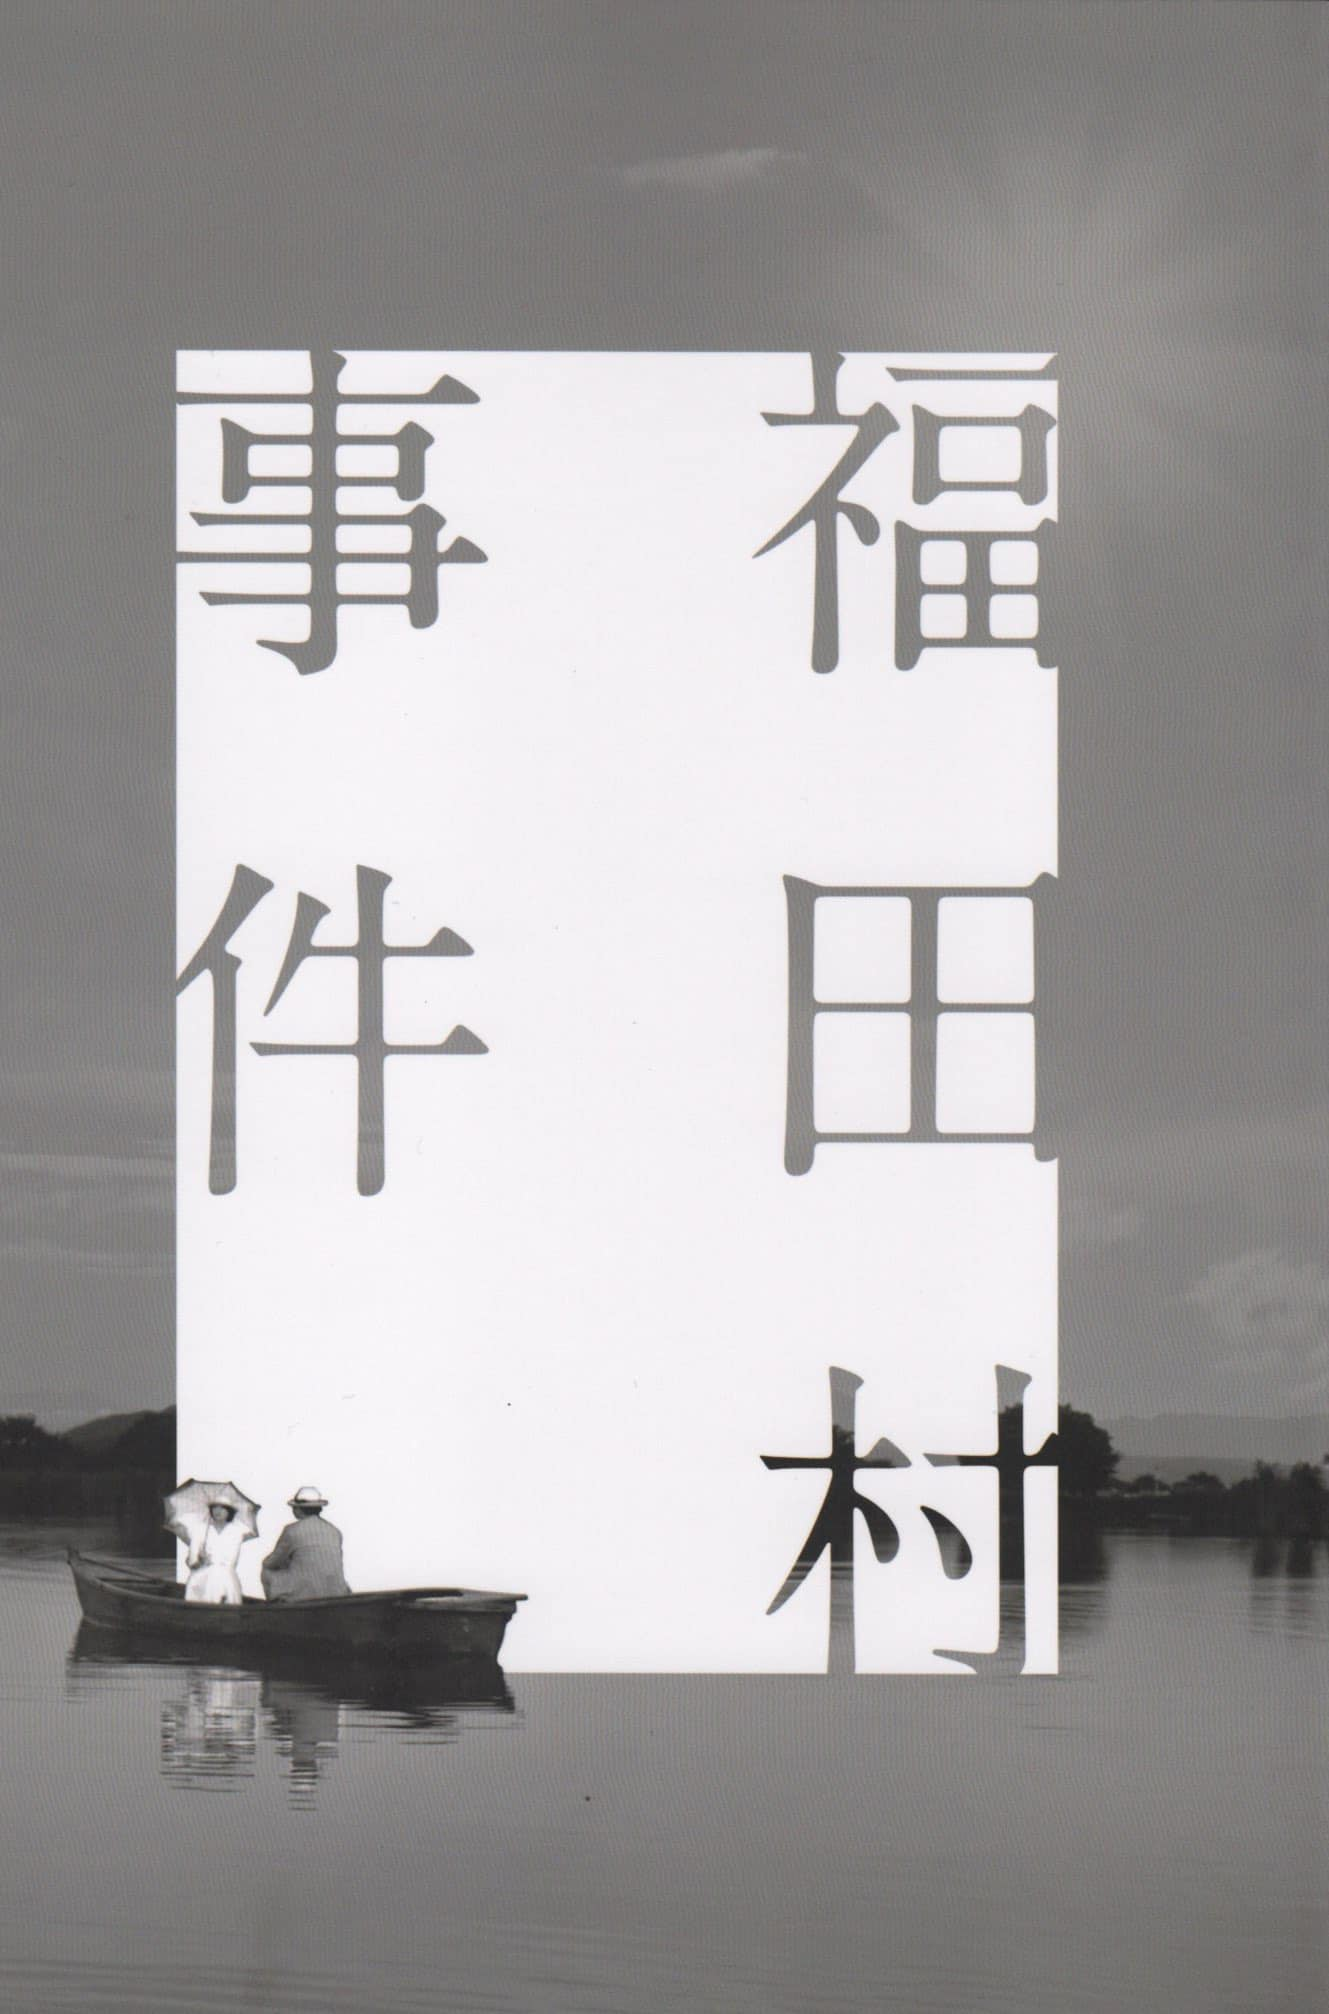
\includegraphics[width=\linewidth]{pictures/2023/10/20231021_163633_001.jpg}
\end{minipage}
\end{center}

\subsection*{2023年10月25日 23:43}
\addcontentsline{toc}{subsection}{2023年10月25日 23:43}

\url{https://www.un.org/sg/en/content/sg/statement/2023-10-24/secretary-generals-remarks-the-security-council-the-middle-east-delivered}

以下はグテーレス国連事務総長の発言です。

”Even war has rules.

We must demand that all parties uphold and respect their obligations under international humanitarian law;

……….

The protection of civilians is paramount in any armed conflict.

Protecting civilians can never mean using them as human shields.

Protecting civilians does not mean ordering more than one million people to evacuate to the south, where there is no shelter, no food, no water, no medicine and no fuel, and then continuing to bomb the south itself.

I am deeply concerned about the clear violations of international humanitarian law that we are witnessing in Gaza.

Let me be clear:  No party to an armed conflict is above international humanitarian law.”

名指しは避けられていますが、ハマスが民間人をどう利用しているのか(using civilians as human shields)、イスラエルが民間人に何を指示しているのか(ordering people to evacuate to the south)、その指示自体無謀である上更に、to bomb the south が続けられている事。これらのことを世界中が知っています。

国際人道法(international humanitarian law)そのものを読んだことはありませんが、パレスチナの言い分、イスラエルの言い分、双方に関わるあらゆる言い分を超えて、今、humanitarian activitiesは何よりも優先されるべきものであるはずだと、（強く）同意します。欧米各国が「テロへの報復」を合唱し、「人道1st」になっていない事に、どうして？という気持ちを禁じ得ません。

\#Guterres \#UN \#Israel \#Gaza \#Hamas \#security \#humanitarian

\paragraph{リンク}
\url{https://www.un.org/sg/en/content/sg/statement/2023-10-24/secretary-generals-remarks-the-security-council-the-middle-east-delivered}

\section{11月}

\subsection*{2023年11月09日 01:19}
\addcontentsline{toc}{subsection}{2023年11月09日 01:19}

\#TED で偶然見かけたものですが、固唾を呑んで聞くことになりました。

モニカ・ルインスキーさんは、当時の米国大統領との大統領執務室におけるスキャンダル、二人の極めてpersonalな事であったはずのintimateな行為が、ネットを通して地球規模で晒された、その当人です。私は当時、クリントン大統領にばかり注目していて、その様な恥を晒され信頼も全て失うことになってしまった彼女の事について考えた事はありませんでした。

全てにおいて絶望的だと感じていたことでしょう。私たちの想像をゆうに超える出来事だっただろうと思います。御両親が、寝室に一晩中一緒にいてくれた事や、シャワーの時もドアを開け放して、彼女を一人にさせない様にされていた事など、御両親の気持ちもどんなに苦しかったことかと推察します。

丁度インターネットが動き始めた頃の出来事です。そのしばらく前であったならば、当事者間、学校内、コミュニティー内部など、localな周辺でおさまっていた様なことが、globalな規模で晒される様になった最初の出来事でした。当時の人類は、起きる事柄を予測できなかったでしょうし、またこの様な事態に対応する知恵を持っていなかったとは言えるかもしれません。しかし、インターネットがインフラとして普及定着した現在においても尚、事態は改善されるどころか、SNSの普及もあって、更に深刻な被害を被るケースが後を絶たない状況です。

最後に次の様にしてお話を終えていらっしゃいます。

I'd like to end on a personal note.

In the past nine months, the question I've been asked the most is "Why?"Why now?

（略）

The top-note answer was and is "Because it's time."

Time to stop tiptoeing around my past, time to stop living a life of opprobrium and time to take back my narrative.

It's also not just about saving myself.

Anyone who is suffering from shame and public humiliation needs to know one thing:You can servive it.

I know it's hard.

It may not be painless, quick or easy, but you can insist on a different ending to your story.

Have compassion for yourself.

We all deserve compassion, and to live both online and off in a more compassionate world.

Thank you for listening.

彼女の I know it’s hard. It may not be painless,quick or easy. という共感の言葉は、anyone who is suffering from shameにとって、とても大きな説得力をもって響くことでしょう。そして彼女が、彼女自身の物語（人生）を取り戻す、今がその時（Why now? … Because it’s time.）なのだと、力強く話す姿を見る時、You can servive it. … you can insist on a different ending to your story. これは前向きな、希望を感じさせる言葉として、本当に力強く伝わってきます（dream などではなくて、insist on なのですから）。compassionをfor yourselfに …、to live in a more compassionate world …は、今日のインターネット社会に投げかけられた、一人ひとりが大切にするべきキーワードですね。

\paragraph{リンク}
\url{https://youtu.be/H_8y0WLm78U?si=vgtPxtG_EpsOJJ5Z}

\subsection*{2023年11月13日 19:09}
\addcontentsline{toc}{subsection}{2023年11月13日 19:09}

「\#トランジスタ技術」（以下「トラ技」）は、\#CQ出版 の月刊誌で、私も学生だった頃から愛読者でした。学生の頃には、CQ出版の「トラ技」、同じCQ出版の「interface」（黒い表紙だった頃の物です）、共立出版の「bit」の3冊は、毎月発売日の1日、2日ほど前には、生協の書籍部に足を運んで楽しみにしていたという記憶があります。

この雑誌「トラ技」はとても分厚い雑誌なのですが、前の1／3の厚さの部分は広告で、真ん中に実際のその月の記事が1／3あって、後ろの1／3はまた広告のページとなっています。いや、記事1／3は多すぎるかもしれません。前の35\%が広告、真ん中の30\%が記事、後ろの35\%が広告という割合の方が近かったかもしれません。（過去形で言っているのは、近年のトラ技は広告が減って薄くなってしまっているからです。）私は学生の頃には、カッターを使って前の広告部分と後ろの広告部分を切り捨てて、真ん中の部分だけを積ん読していたものです。（でも当時はインターネットも無かったので、この広告の部分こそが大切な情報源なんだと言っていた人もいました。）

さて、この番組「\#世にも奇妙な物語」ですが、「‘23秋の特別編」の第4話がとてもシュールな「トラ技の圧縮」（真ん中の記事部分だけを残す作業）の物語になっていて、私の様に身に覚えのある者にとって、抱腹絶倒なお話になっていました。話の中では「トランジスタ技術」の雑誌そのものが使われていて、他にこの様な雑誌はなかった、唯一無二の存在だったんだと納得してしまいました。

\paragraph{リンク}
\url{https://www.fujitv.co.jp/kimyo/202311.html#num20231103}

\subsection*{2023年11月18日 21:56}
\addcontentsline{toc}{subsection}{2023年11月18日 21:56}

「\#朽ちていった命 ー被爆治療83日間の記録ー」（\#新潮文庫）を読みました（一気に）。

これはNHK取材班が、茨城県 \#東海村 にあった核燃料加工施設 \#JCO で1999年に起こした「東海村臨界事故」で犠牲になった大内久氏の被爆から亡くなられるまでの有り様を、医師、看護師、遺族に取材してまとめられたものです。

バケツの中で \#ウラン（この時のウランの量は千分の一グラム＝１mgだったと言う事です）を溶かして、その溶液を別の容器に移す作業中の事です。大内氏は、先輩がバケツから流し込むウラン溶液を受けるロウトを支える作業（手で支えている）を受け持っていたそうです。七杯目のバケツのウラン溶液が流し込まれ始めた時、容器の中では \#臨界 に達し（ \#核分裂 の連鎖反応が始まり）、この時放射された \#中性子 によって \#被爆 したという事故です。

当時ニュースの情報を聞いて真っ先に思ったのは、バケツ？、ロウト？、人手でウラン溶液を？そんな事で良かったの？と言う一連のハテナばかりがありました。今回この本を読んで、現代の最新医療が手探りで必死に施される中で、実際には被爆した人の体が、83日の間にどんどん「朽ちて」いって死に至る様をまざまざと知る事になり、言葉では言い表せない衝撃を受けました。

\paragraph{リンク}
\url{https://www.shinchosha.co.jp/book/129551/}

\subsection*{2023年11月25日 22:54}
\addcontentsline{toc}{subsection}{2023年11月25日 22:54}

\url{https://x.com/bReCaG48/status/1728229013678961118?s=20}

\paragraph{写真}
\begin{center}
\begin{minipage}{0.70\linewidth}
\centering
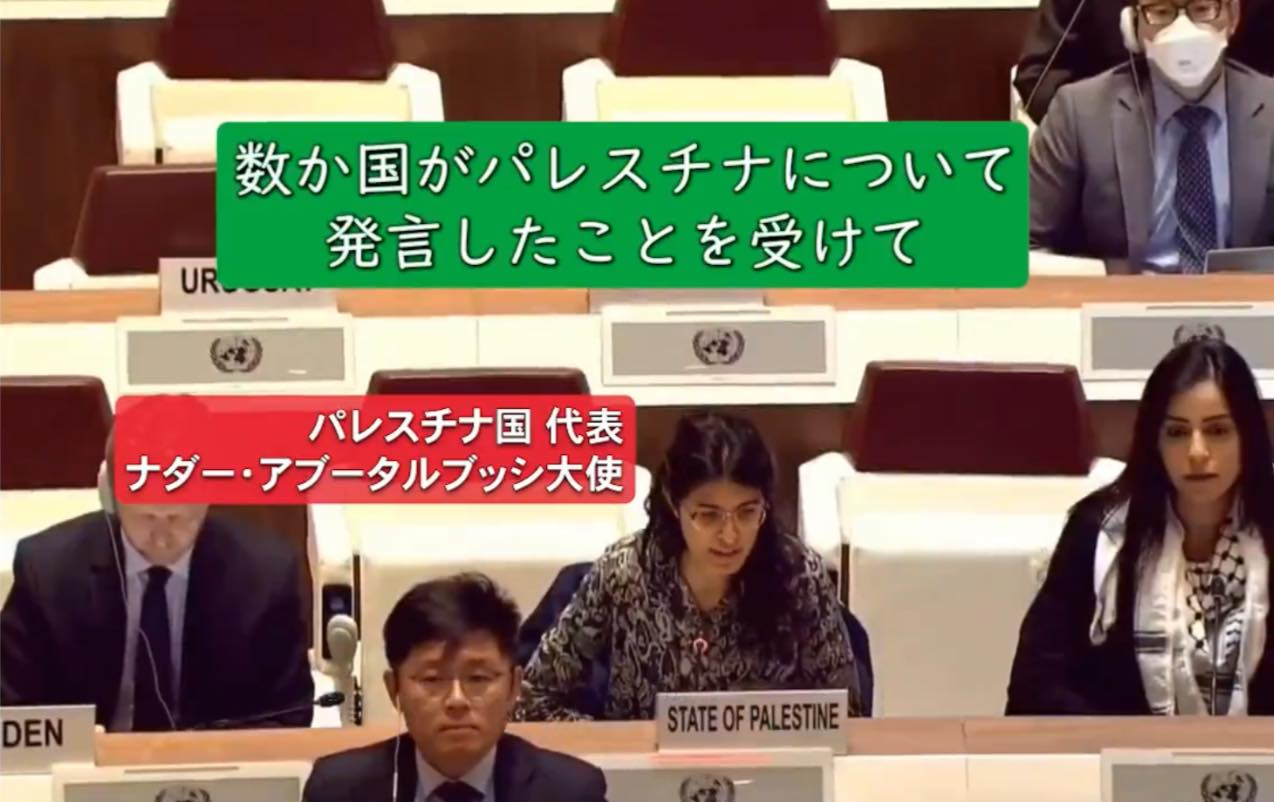
\includegraphics[width=\linewidth]{pictures/2023/11/20231125_225408_001.jpg}
\end{minipage}
\end{center}

\subsection*{2023年11月26日 14:59}
\addcontentsline{toc}{subsection}{2023年11月26日 14:59}

ネット上で見かけた（ \url{https://x.com/kiwamu_watanabe/status/1728180828260434023?} ）もの（\#Xmas ネタとして定番らしい）です。控えておこうと思って、勝手ながら「\#TeX で清書」させていただきました。

\paragraph{写真}
\begin{center}
\begin{minipage}{0.70\linewidth}
\centering
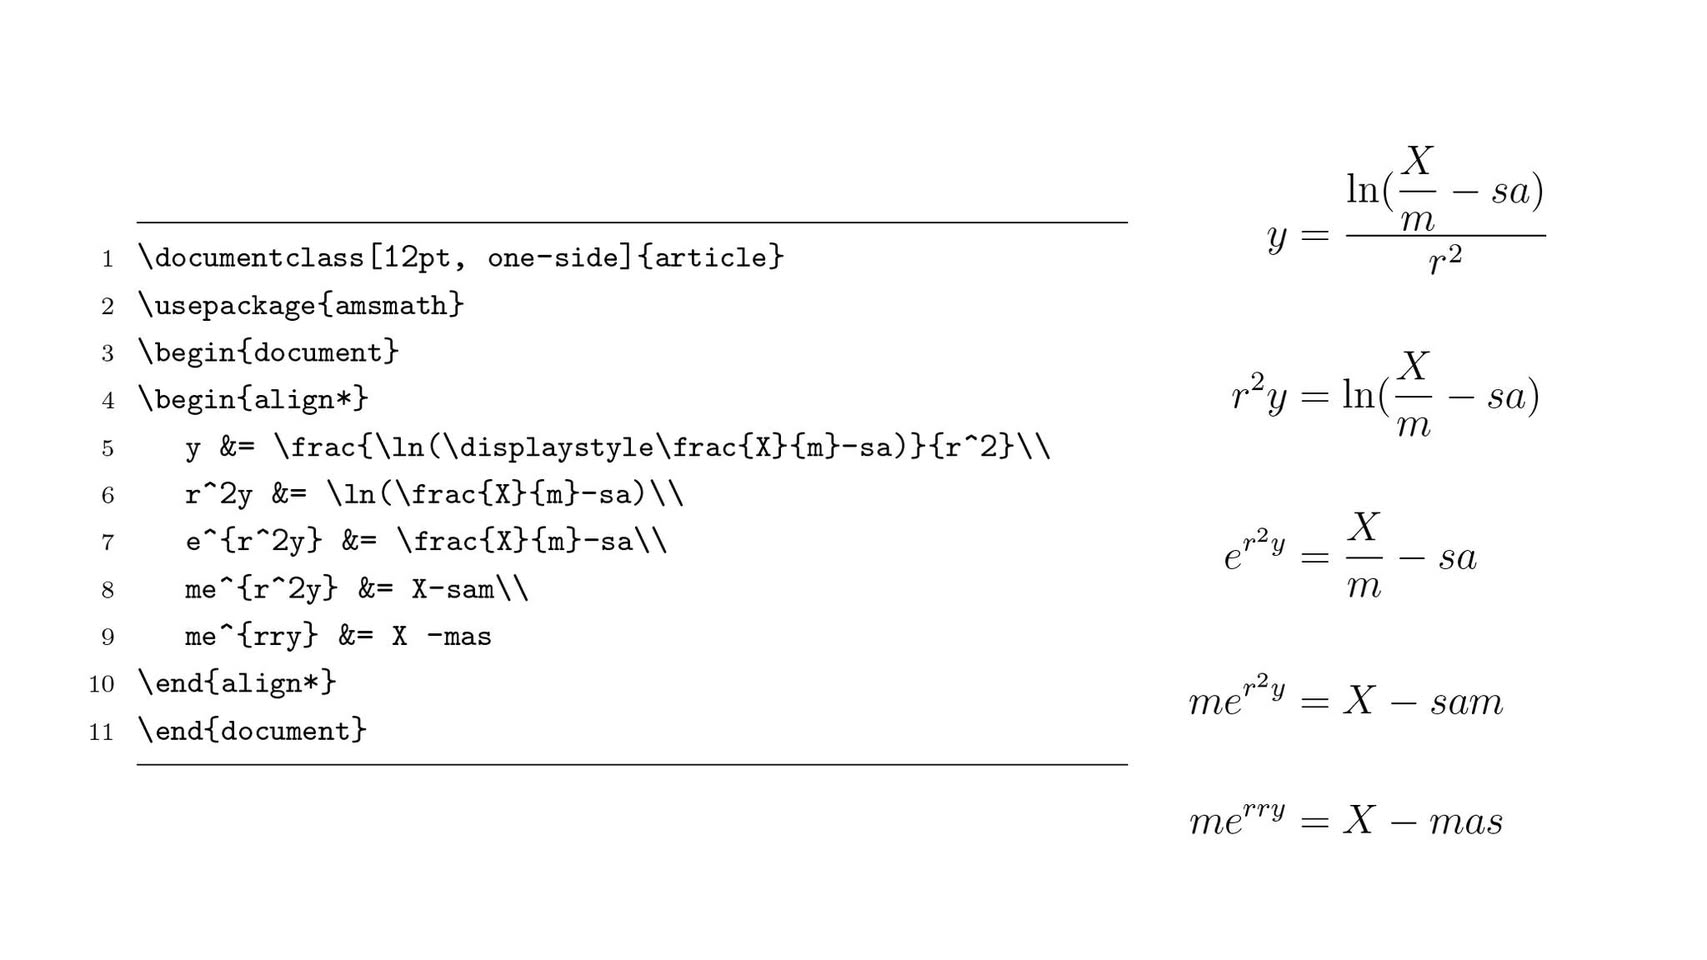
\includegraphics[width=\linewidth]{pictures/2023/11/20231126_145957_001.jpg}
\end{minipage}
\end{center}

\subsection*{2023年11月30日 18:57}
\addcontentsline{toc}{subsection}{2023年11月30日 18:57}

千葉県教育委員会の「見識」に呆れると共に、怒りさえ覚える。

教員が塾講師のやり方を見て学ぶ機会が設けられたという事であれば、それはあっても良いとは思うが。このやり方は、、、、教育者の発想ではないでしょう。そもそもこの板書は、高校生以上になら許せるかもだが、小学生には見せたくない。「僕もこんな綺麗な字を書けるようになりたい」と思わせるような、とめはねを意識した丁寧な字を黒板に並べて欲しい。算数なのだからは言い訳にならない。これは枝葉末節ではないのです！（小学校の）教員であったならば、板書はおそらく多くが意識している事だろうと思います。

\paragraph{リンク}
\url{https://news.yahoo.co.jp/articles/37e7af0b0011629ae478be88684220b017740120?source=fb}

\section{12月}

\subsection*{2023年12月04日 08:30}
\addcontentsline{toc}{subsection}{2023年12月04日 08:30}

今朝12/4 \#NHK の「おはよう日本」で放送されていた、\#ガザ地区 の難民キャンプにいる医学生マルワさん（21）の訴えです。（情報源は \#ユニセフ、国連児童基金）

I pray that they could look at us as humans,

not just political situations and political conflicts.

We have lives.

And we should be able to live our lives.

政治的状況や政治的対立ではなく、

人間として見てほしい。

自分の人生を生きることができるべきだ。

\subsection*{2023年12月10日 05:03}
\addcontentsline{toc}{subsection}{2023年12月10日 05:03}

ガザにおける即時の人道的停戦を要求しているのに、、、

US🇺🇸はどうして堂々とこんなことができるのか？（UK🇬🇧は棄権。JP🇯🇵は今回珍しくアメリカに追従していない。）「これからも非人道的な諸行、殺りくを続けて行くべきだ」と主張しているのと同じ事です。その国の品格を疑うというか何というか、、、アメリカもやっぱり、そんな国だったんだね（うかつにも失念しておりました）。9.11に対する報復の正当性を、ここでも主張していらっしゃるのでしょうか？イスラエル🇮🇱とその支持者への忖度でしょうか？イスラエルと同じ立ち位置に立っているという事を、国際的に、明確な立場として、改めて表明されているのですね。ロシア🇷🇺と同様、アメリカも世界から孤立していくのではないかと心配する声もあります。(日本はそんなのに追従していっていいのか？)

それにしても、「拒否権」と呼ばれる手段が決定する事について、同意できた例は思い当たりません。

\#StopGenocideInGaza \#CeasefireNow

\paragraph{写真}
\begin{center}
\begin{minipage}{0.70\linewidth}
\centering
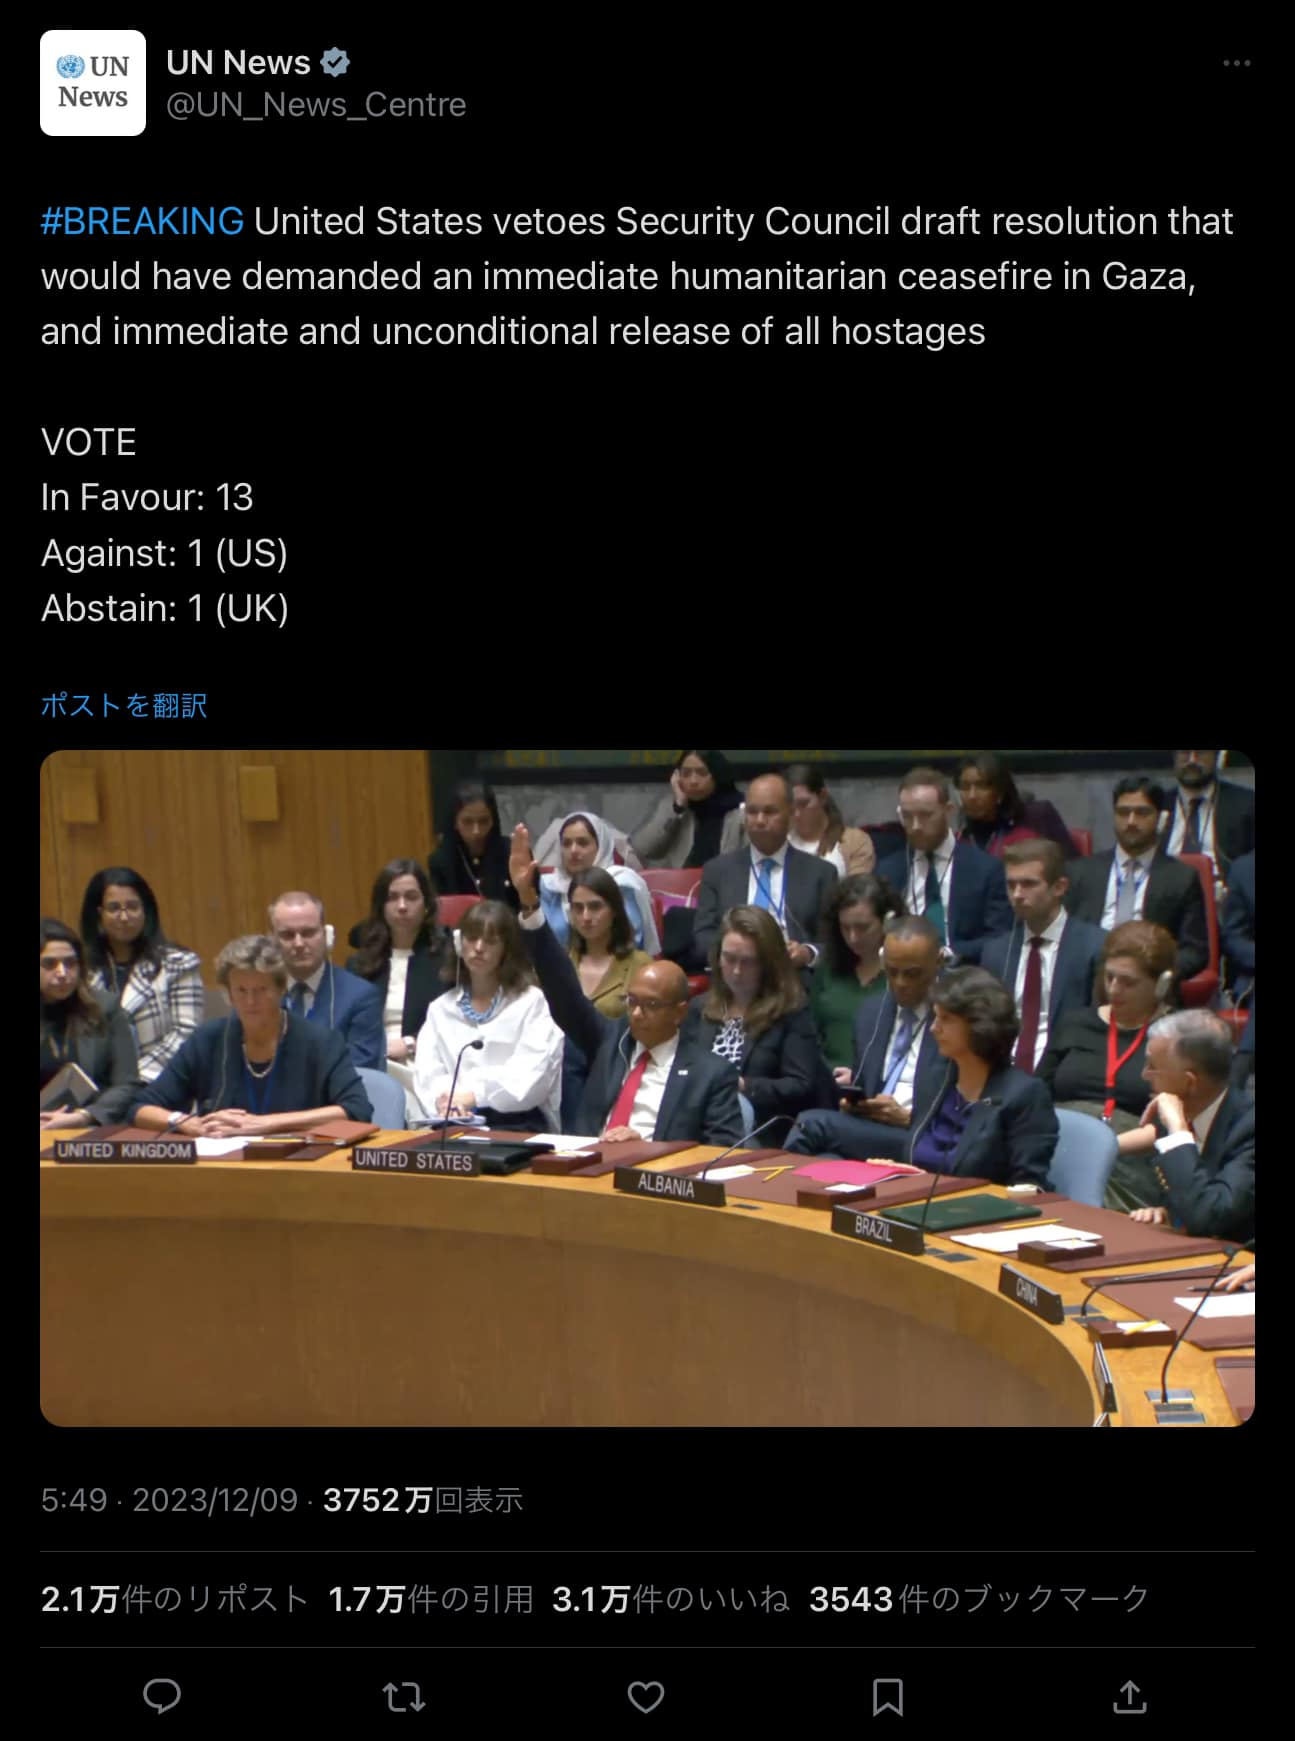
\includegraphics[width=\linewidth]{pictures/2023/12/20231210_050312_001.jpg}
\end{minipage}
\end{center}

\subsection*{2023年12月18日 17:10}
\addcontentsline{toc}{subsection}{2023年12月18日 17:10}

\url{https://x.com/haemosun/status/1736188628433600781?s=20}

私は大きな米農家ではありません。小さな面積の田んぼを持っているので作ってもらっています。昨年までは面積相応の僅かな収入がありました。ところが今年の決算ではマイナスの収入になっていました。つまり「お米を生産するとは支出を伴うこと」という事態になっています。私の所有する田んぼの面積は小さいので被害もそれなりの金額で済んでいますが、広い面積の田んぼを持っていらっしゃる家ではどうなのだろうかと心配です。日本の米の自給率が小さいのに、この状態では農家は存続できないのではないかと危惧します。つい暫く前にも、外国産の肉の輸入が盛んに行われている中、畜産農家でも同様の状況、廃業せざるを得ない状況があるという報道があった事を記憶しています。いずれも行政は傍観しているだけなのか気にしています。

\paragraph{写真}
\begin{center}
\begin{minipage}{0.70\linewidth}
\centering
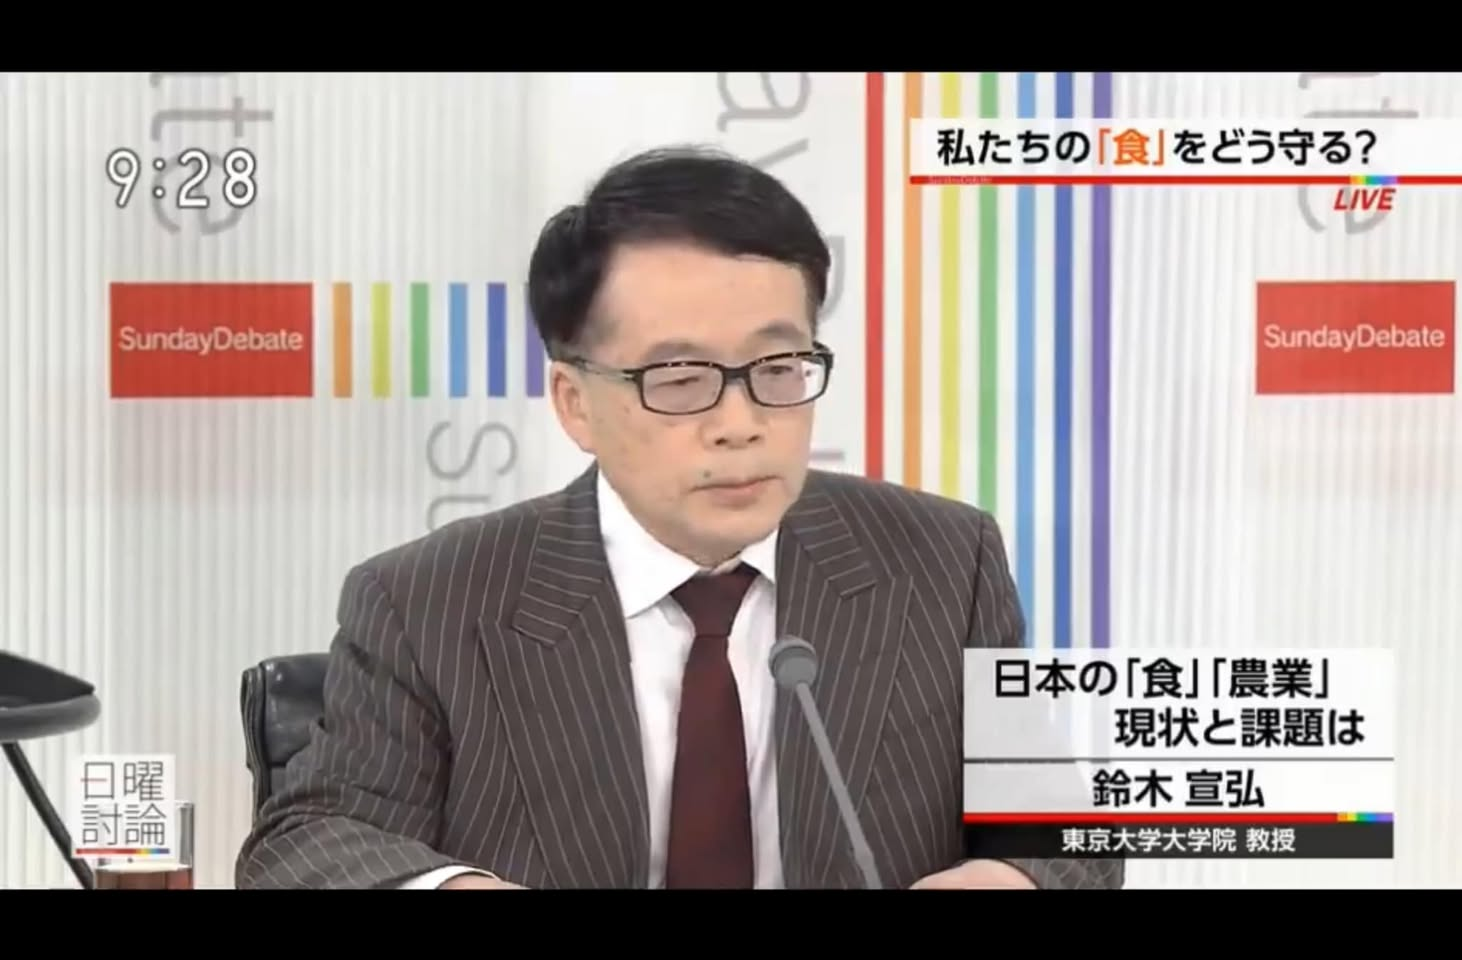
\includegraphics[width=\linewidth]{pictures/2023/12/20231218_171025_001.jpg}
\end{minipage}
\end{center}

\subsection*{2023年12月19日 12:42}
\addcontentsline{toc}{subsection}{2023年12月19日 12:42}

\url{https://x.com/nhk_kurogen/status/1736703606227681342?s=61&t=5VtsOkpki6juEjPXsBq8hg}

山田太一さんの代表的な作品に一貫する、山田太一さんの眼差しに気付かされる番組だった。

コンプレックスを抱えている若者、社会から疎まれ声を上げる事をはばかられる老人たち、車椅子などハンディを持っている人達、それらの視点に立って代弁している作品たち。昭和の香りがするとは言え、問題意識として、決して過去そんな時代だったとして片付けられない、現代にも問いかけられ続けている問題でした。

（弱者から見た）こうした視点を忘れずに、意識し続ける事を大切にしたいという気持ちになりました。

\#クローズアップ現代 \#山田太一 \#クロ現 \#NHK

\paragraph{写真}
\begin{center}
\begin{minipage}{0.70\linewidth}
\centering
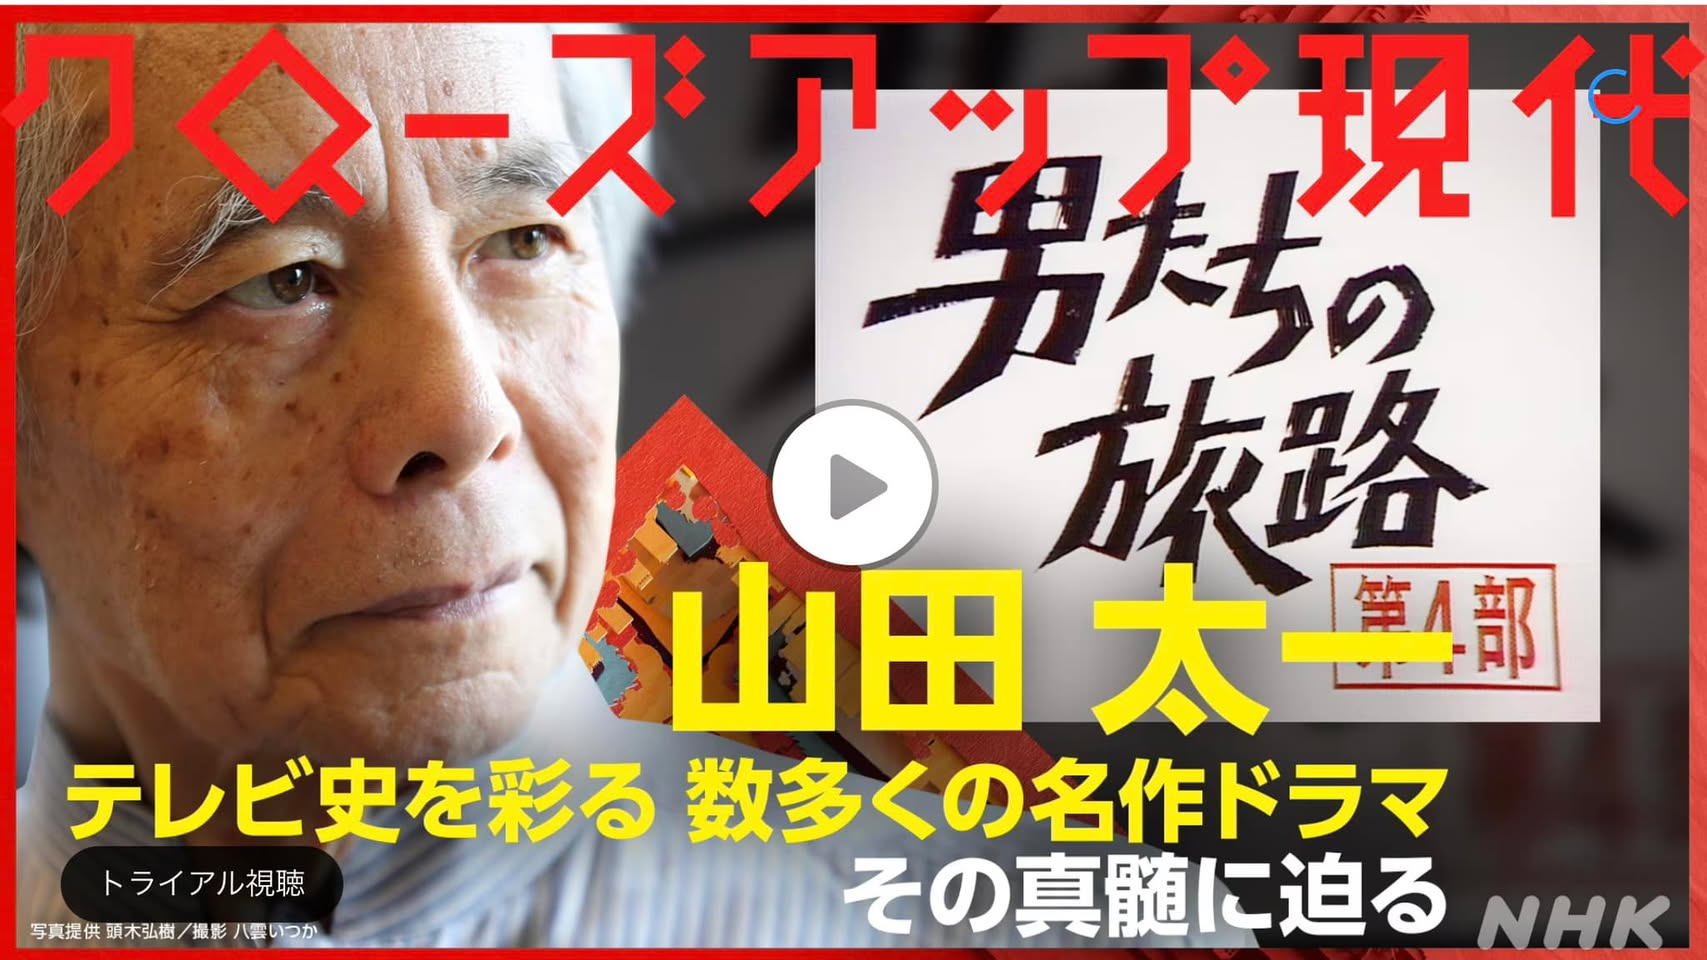
\includegraphics[width=\linewidth]{pictures/2023/12/20231219_124231_001.jpg}
\end{minipage}
\end{center}

\subsection*{2023年12月22日 06:56}
\addcontentsline{toc}{subsection}{2023年12月22日 06:56}

\url{https://www.nhk.or.jp/minplus/0121/topic049.html?cid=gendaihk-tw-202312211903}

1、ハマスによるインスラエルへのテロ攻撃（10／7）の５日前に、UNRWA（国連パレスチナ難民救済事業機関）ラザリーニ事務局長がNHKの取材に「今年に入って暴力の応酬が激化している。このままでは危機が再燃する」と答えている。一方でアメリカのサリバン大統領補佐官が、ハマスの攻撃の直前に「中東はここ２０年来、かつてないほど静かだ」との認識を示していた。このギャップは、国際社会がこの地域からの明確なシグナルを受け止められていなかった事を物語っている。

2．イランの映画監督モフセン・マフマルバフ氏「この20年間に空から爆弾を落とすより教科書を落としていたら、アフガニスタンはこうはなっていなかった。地面に地雷をまくより麦をまいていれば、アフガニスタンはこうならなかった」

3．国連のグテーレス事務総長が国連安全保障理事会での発言「ハマスによる攻撃は理由もなく起きたわけではない」これに対してイスラエルは強く反発し事務総長の辞任要求にまで。

4．国谷裕子氏「誰に対してもフェアに問う。問うべき事をしっかりと問う。言葉を通して真実を浮かび上がらせる事を目指してきた。その時自分の中に偏見や思い込みがないかという事に常に気をつけながら、聞くべき事を聞く、繰り返し角度を変えて聞く事が大事」グテーレス事務総長は、イスラエルとパレスチナとの中立ではなく、事実に基づいた発言を、国際社会へのメッセージとして発信した。メディアの取るべき姿勢と重なるものがある。

国谷裕子氏の、アラファト議長やイスラエルの指導者に対する、忖度のない率直な問いかけインタビューは、近年では耳にしたことのないものでした。グテーレス事務総長の事実に基づく発言にイスラエルが逆ギレした様に、国谷氏による、当時のS官房長官に対する率直な問いかけが、当時のAB政権権力者の逆ギレに繋がり、番組を降板させられる事になったのは7年前の事でした。

\#クローズアップ現代 \#国谷裕子 \#クロ現 \#NHK \#国谷

\paragraph{写真}
\begin{center}
\begin{minipage}{0.70\linewidth}
\centering
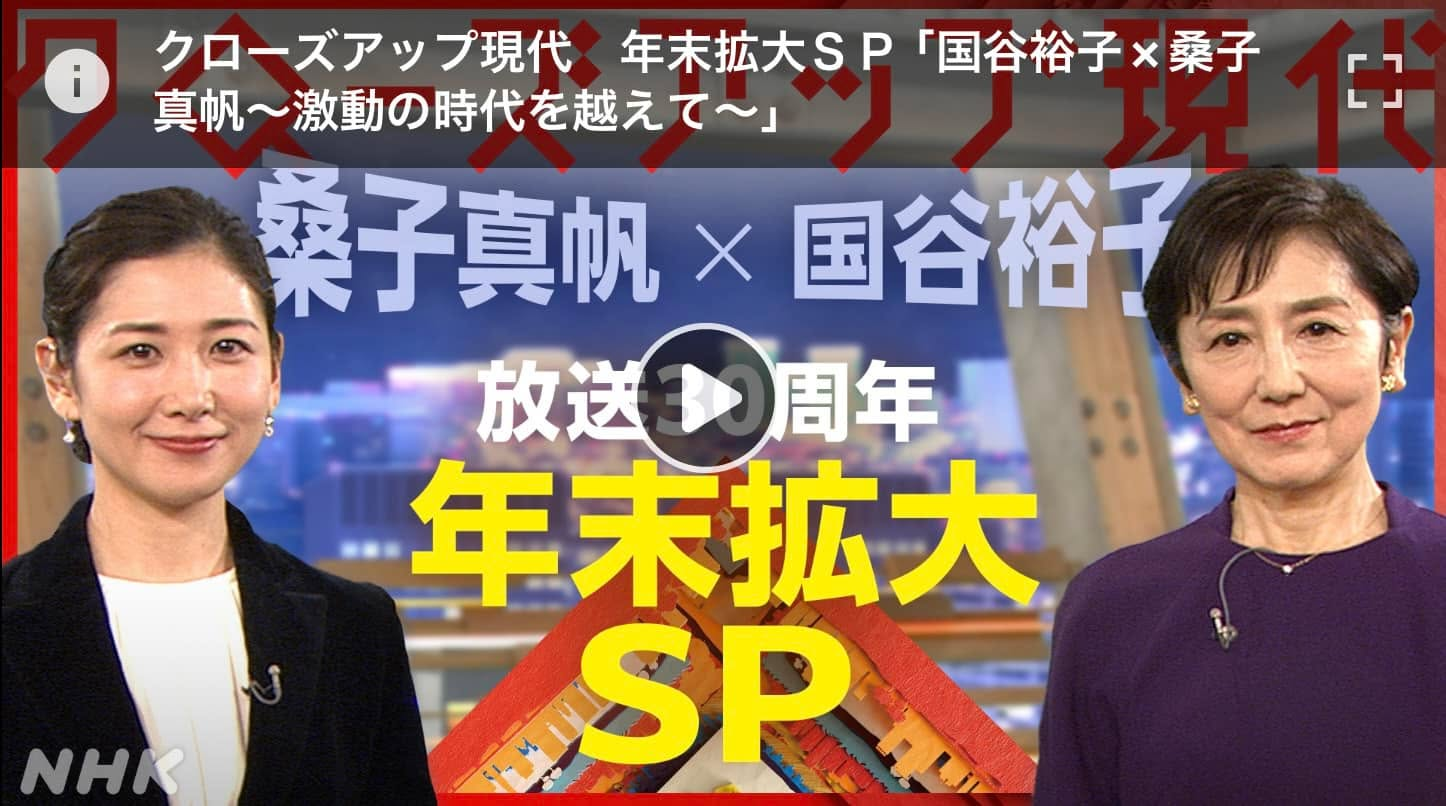
\includegraphics[width=\linewidth]{pictures/2023/12/20231222_065620_001.jpg}
\end{minipage}
\end{center}

\subsection*{2023年12月24日 16:13}
\addcontentsline{toc}{subsection}{2023年12月24日 16:13}

\url{https://x.com/ummadel473708/status/1738649676721602851?s=61&t=5VtsOkpki6juEjPXsBq8hg}

そうだよ。おかしいよ。

パレスチナの人々に生きてと言うためには、投票しないといけないの？そもそも多数決で決める様な類のことなの？（拒否権を行使する国があるから、多数決ですらないのだけど）

Why are you voting on?

Why is that a vote?

Why is that even an ask?

Why are we asking people to save our families, children , to save  any human being?

人が生きるか死ぬかについて、真面目な顔で正装して集まって、円卓で投票して決めようとしている。この図は、、、。この世界は異常だ。麻痺してしまっている。そもそも国連安保理の全会一致がなければ動けない事なのか。

\#StopGenocideInGaza \#CeasefireNow

\paragraph{写真}
\begin{center}
\begin{minipage}{0.70\linewidth}
\centering
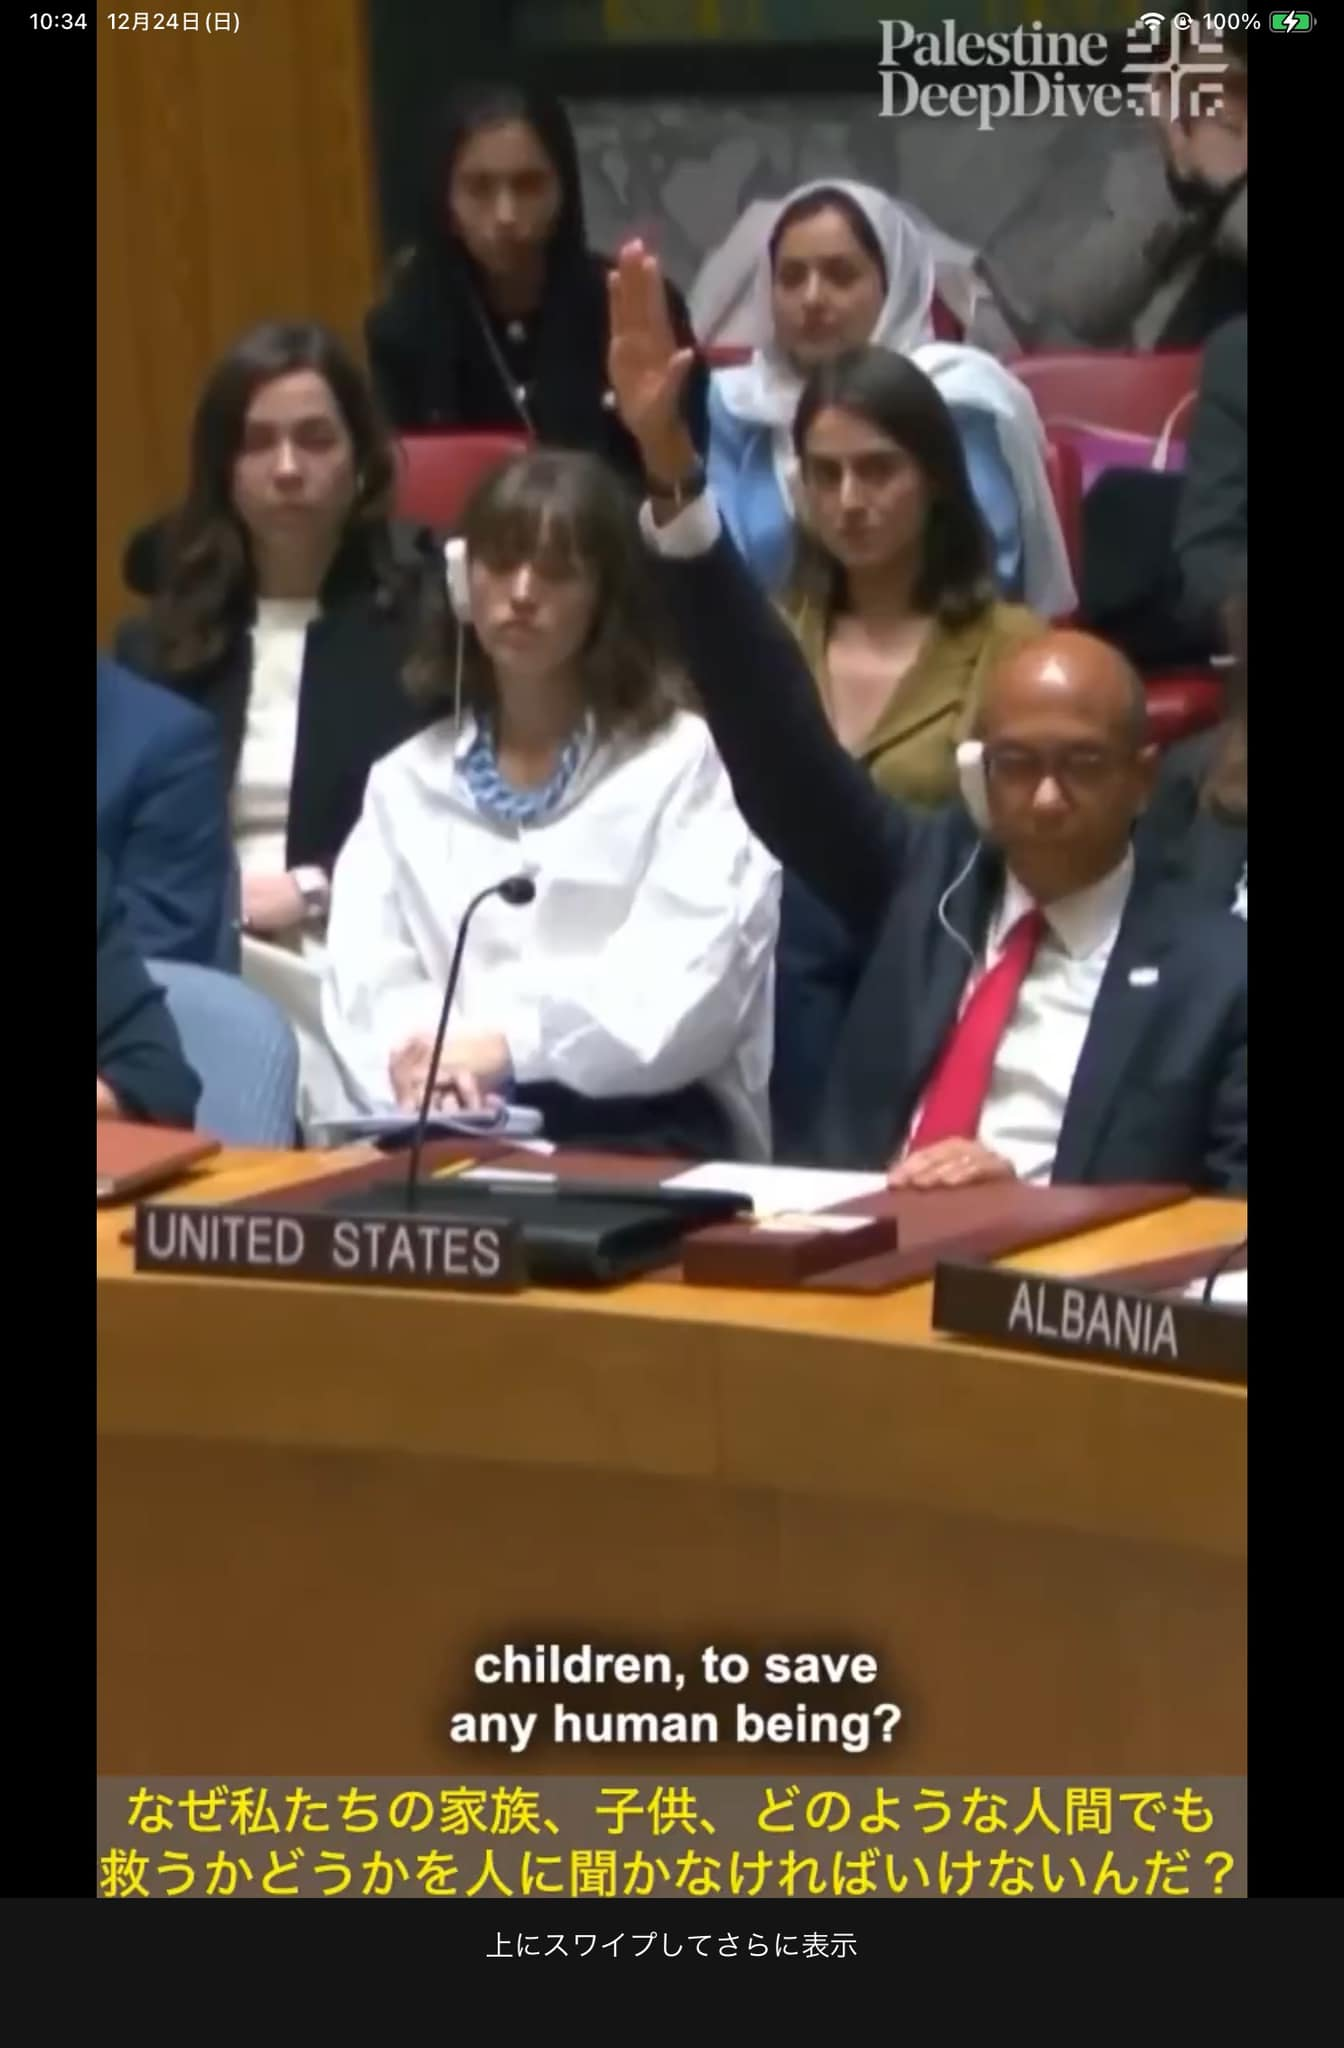
\includegraphics[width=\linewidth]{pictures/2023/12/20231224_161305_001.jpg}
\end{minipage}
\end{center}

\subsection*{2023年12月28日 02:52}
\addcontentsline{toc}{subsection}{2023年12月28日 02:52}

\url{https://x.com/picturesfoider/status/1739567726174089504?s=61&t=5VtsOkpki6juEjPXsBq8hg}

ほんとだー、８に見える

今まで気づかなかったよ

\paragraph{写真}
\begin{center}
\begin{minipage}{0.70\linewidth}
\centering
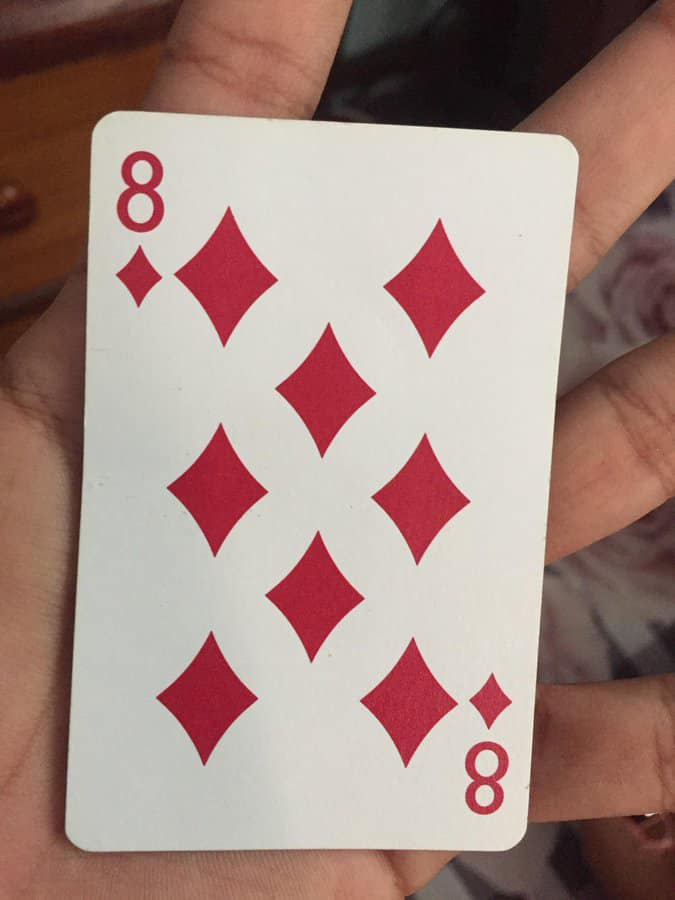
\includegraphics[width=\linewidth]{pictures/2023/12/20231228_025259_001.jpg}
\end{minipage}
\end{center}

\subsection*{2023年12月28日 06:12}
\addcontentsline{toc}{subsection}{2023年12月28日 06:12}

\url{https://www.u-tokyo.ac.jp/focus/en/press/z0508_00323.html}

理由を理解したいと思うんだけど、

何をどう勉強したら、理解できたという気持ちになれる？

（量子コンピュータについても同様に気にしているのだが. ボケ防止に効果的かと思っていたけど、、、諦めた方がいいという声も心の中では聞こえている．）

\paragraph{リンク}
\url{https://www.u-tokyo.ac.jp/focus/en/press/z0508_00323.html}

